% !TeX program = xelatex
% 编译顺序：xelatex main -> bibtex main -> xelatex main -> xelatex main
\documentclass[11pt,a4paper,fontset=windows]{ctexart}

\usepackage[left=2.6cm,right=2.6cm,top=2.8cm,bottom=2.8cm]{geometry}
\usepackage{amsmath,amssymb}
\usepackage{graphicx}
\usepackage{tikz}
\usetikzlibrary{arrows.meta,positioning,shapes.geometric,calc,fit,backgrounds,patterns}
\usepackage{pgfplots}
\pgfplotsset{compat=1.18}
\usepackage{booktabs}
\usepackage{multirow}
\usepackage{array}
\usepackage{caption}
\captionsetup{font=small,labelfont=bf,labelsep=quad}
\captionsetup[table]{skip=3pt}
\usepackage{enumitem}
\setlist{nosep,leftmargin=2em}
\usepackage{microtype}
\usepackage{xcolor}
\usepackage{algorithm}
\usepackage{algpseudocode}
\floatname{algorithm}{算法}
\usepackage[colorlinks=true,linkcolor=black,citecolor=black,urlcolor=blue!55!black]{hyperref}
\usepackage{url}

\linespread{1.18}
\setlength{\emergencystretch}{2em}

\definecolor{ink}{HTML}{22303C}
\definecolor{slate}{HTML}{4A6572}
\definecolor{mist}{HTML}{E9EEF1}
\definecolor{teal}{HTML}{6E8F8C}
\definecolor{sand}{HTML}{C9B79C}
\definecolor{alert}{HTML}{B23A48}

% 占位标记：稿件定稿前统一检索并替换
\newcommand{\needdata}[1]{\textcolor{alert}{[待补数据：#1]}}
\newcommand{\needcheck}[1]{\textcolor{alert}{[待核：#1]}}
\newcommand{\ph}{\,--\,}

% 唯一数字入口：所有实验数值宏在此定义
% =====================================================================
% results.tex — 单一宏源（中文版）
% 初稿中所有精度数值均为占位符 \ph；工程实测值（分块敏感性、显存/吞吐）
% 只在对应表格使用，且已注明来源。第二部分的真实结果文件到位后，
% 只改本文件即可让正文与图表同步更新。
% =====================================================================

\providecommand{\ph}{\textemdash}
\newcommand{\resultsavailable}{1}      % 1 = 真实结果已注入
\newcommand{\qualitativeavailable}{0}  % 1 = 定性图已就位

% ---------- 工程实测：分块敏感性（同一权重、仅改分块） ----------
\newcommand{\tilingN}{40}
\newcommand{\tilingDefault}{384}
\newcommand{\tileA}{0.370}   % 128
\newcommand{\tileB}{0.410}   % 192
\newcommand{\tileC}{0.480}   % 256
\newcommand{\tileD}{0.644}   % 384
\newcommand{\tileE}{0.643}   % 448
\newcommand{\tileF}{0.655}   % 512
\newcommand{\tileG}{0.593}   % full 640x1280

% ---------- 工程实测：显存档位 ----------
\newcommand{\vramSix}{0.89}
\newcommand{\spsSix}{3.54}
\newcommand{\epochSix}{197.5}
\newcommand{\vramEight}{1.227}
\newcommand{\spsEight}{3.10}
\newcommand{\epochEight}{225.6}
\newcommand{\gpuName}{RTX 4060 Laptop 8\,GB}

% ---------- 划分与权重 ----------
% splitSig 标识“文件清单”（999 例去重后的 stems）；assignmentSig 标识“实际派分”。
\newcommand{\splitSig}{6bdacfb0a71b8196\allowbreak 08dba4cde4382f8d\allowbreak d23fb4a88b72c9b6\allowbreak d151a99ed83bc22a}
\newcommand{\assignmentSig}{7a6fd5819d048e0c\allowbreak cd811c943d616a0f\allowbreak e8738a5c06bc7875\allowbreak 2c66bb38624795f6}
\newcommand{\nTrain}{694}
\newcommand{\nVal}{153}
\newcommand{\nTest}{152}
\newcommand{\nTotal}{999}   % 去重后的有效配对总数；验证集为 \nVal，测试集为 \nTest
\newcommand{\nTrainPatients}{239}
\newcommand{\nValPatients}{50}
\newcommand{\nTestPatients}{49}
\newcommand{\officialTestImages}{200}
\newcommand{\officialTestPatients}{166}
\newcommand{\officialLeakImages}{326}
\newcommand{\officialLeakPatients}{116}
\newcommand{\cleanOfficialImages}{60}
\newcommand{\cleanOfficialPatients}{50}
\newcommand{\leakyTrainImages}{649}
\newcommand{\leakyValImages}{150}

% ---------- 新故事：泄漏 / MTE / 不确定性 / 临床分级（待结果注入） ----------
\newcommand{\leakDiceClean}{0.7243}
\newcommand{\leakDiceLeaky}{0.6870}
\newcommand{\leakDelta}{-0.0373}
\newcommand{\mteDiceMF}{0.7736}
\newcommand{\mteHDMF}{61.85}
\newcommand{\mteClDiceMF}{0.8140}
\newcommand{\mteGainMF}{-0.0013}
\newcommand{\aurocVarMF}{0.639}
\newcommand{\aurocEntropyMF}{0.483}
\newcommand{\aurocTTAEightMF}{1.000}
\newcommand{\qwkMF}{0.131}
\newcommand{\maeMF}{1.105}
\newcommand{\accMF}{0.164}
\newcommand{\diceUpperMF}{0.7584}
\newcommand{\diceLowerMF}{0.7905}
\newcommand{\diceGapMF}{-0.0321}
\newcommand{\mteGainBest}{\ph}
\newcommand{\leakGainBest}{\ph}

% ---------- 独立测试（holdout）：腺体 ----------
\newcommand{\gDiceMF}{0.7749}\newcommand{\gDiceUNet}{0.7119}\newcommand{\gDiceAtt}{0.7771}\newcommand{\gDiceWRCANet}{\ph}\newcommand{\gDicePrior}{0.7640}
\newcommand{\gIoUMF}{0.6372}\newcommand{\gIoUUNet}{0.5644}\newcommand{\gIoUAtt}{0.6452}\newcommand{\gIoUWRCANet}{\ph}\newcommand{\gIoUPrior}{0.6283}
\newcommand{\gClDiceMF}{0.8156}\newcommand{\gClDiceUNet}{0.8531}\newcommand{\gClDiceAtt}{0.8349}\newcommand{\gClDiceWRCANet}{\ph}\newcommand{\gClDicePrior}{0.8539}
\newcommand{\gHDMF}{68.0456}\newcommand{\gHDUNet}{148.0257}\newcommand{\gHDAtt}{118.4399}\newcommand{\gHDWRCANet}{\ph}\newcommand{\gHDPrior}{154.0330}
\newcommand{\gASSDMF}{20.8838}\newcommand{\gASSDUNet}{27.2330}\newcommand{\gASSDAlt}{16.4637}\newcommand{\gASSDWRCANet}{\ph}\newcommand{\gASSDPrior}{21.0490}
\newcommand{\gPrecMF}{\ph}\newcommand{\gRecMF}{\ph}
\newcommand{\gDiceMFci}{\ph}

% ---------- 独立测试（holdout）：睑缘（辅助任务） ----------
\newcommand{\eDiceMF}{\ph}\newcommand{\eDiceUNet}{\ph}\newcommand{\eDiceAtt}{\ph}\newcommand{\eDiceWRCANet}{\ph}\newcommand{\eDicePrior}{\ph}
\newcommand{\eIoUMF}{\ph}\newcommand{\eIoUUNet}{\ph}\newcommand{\eIoUAtt}{\ph}\newcommand{\eIoUWRCANet}{\ph}\newcommand{\eIoUPrior}{\ph}

% ---------- 训练集自评（仅同分布参考，不代表泛化） ----------
\newcommand{\gDiceMFself}{\ph}\newcommand{\gDiceUNetself}{\ph}\newcommand{\gDiceAttself}{\ph}\newcommand{\gDiceWRCANetself}{\ph}\newcommand{\gDicePriortself}{\ph}
\newcommand{\legacyUNetSelfDice}{0.7021}
\newcommand{\legacyUNetSelfIoU}{0.5512}
\newcommand{\legacyUNetSelfClDice}{0.7204}

% ---------- 消融 ----------
\newcommand{\ablFull}{0.7119}
\newcommand{\ablNoClDice}{\ph}
\newcommand{\ablNoDS}{\ph}
\newcommand{\ablNoEyelid}{\ph}
\newcommand{\ablBoundary}{\ph}
\newcommand{\ablRandInit}{\ph}
\newcommand{\ablImageNet}{\ph}
\newcommand{\ablNoIntensity}{\ph}
\newcommand{\ablNoMultiScale}{\ph}
\newcommand{\ablVerticalFlip}{\ph}
\newcommand{\ablFullClDice}{\ph}

% ---------- TTA 与集成 ----------
\newcommand{\ttaOff}{0.7749}
\newcommand{\ttaTwo}{\ph}
\newcommand{\ttaEight}{0.7808}
\newcommand{\ensSingle}{\ph}
\newcommand{\ensFive}{\ph}

% ---------- 统计检验 ----------
\newcommand{\pMFUNet}{5.44e-20}
\newcommand{\pMFAtt}{0.0161}
\newcommand{\pMFWRCANet}{\ph}
\newcommand{\pMFPrior}{0.714}
\newcommand{\holmAlpha}{0.05}


\title{\bfseries 面向公开基准的睑板腺分割：\\[2pt]
患者级泄漏、分块混杂与不确定性引导复核}
\author{第一作者$^{1}$\thanks{通信作者：待填（姓名、邮箱、单位地址）。}\quad
第二作者$^{1}$\quad 第三作者$^{2}$\\[4pt]
{\small $^{1}$待填单位一，城市，邮编\quad $^{2}$待填单位二，城市，邮编}}
\date{}

\begin{document}
\maketitle

\begin{center}
\footnotesize\color{gray}
稿件状态：基准稿 v0.4（MGD-1K 患者级划分 + 工程基线 v2.3.0）\quad|\quad 实验数值由统一训练与患者级独立测试注入\quad|\quad
作者、单位、基金、伦理批号均为待替换项
\end{center}

\vspace{-0.6em}

\tableofcontents
\newpage

\begin{abstract}
睑板腺功能障碍（MGD）的红外睑板影像分割已有大量深度学习方法，但公开基准的可比性仍受三类问题影响：图像级划分使同一患者跨训练与测试、分块推理参数未被报告、像素指标与临床 Meiboscore 脱节。本文在公开 MGD-1K 上建立一个患者独立、可复现的基准：\nTotal{} 例去重配对来自 338 名受试者，按患者分为 \nTrain/\nVal/\nTest{}（\nTrainPatients/\nValPatients/\nTestPatients{} 名患者），并公开划分文件与 assignment signature。

我们首先量化一个被忽视的泄漏：官方 \officialTestImages{} 例 Meiboscore 测试清单含 \officialTestPatients{} 名患者，而其余 800 例中有 \officialLeakImages{} 例来自同一批患者；即使在患者级训练集中，仍有 \officialLeakPatients/\officialTestPatients{} 名测试患者出现。随后，在同一预处理、同一患者级划分、同一损失与同一推理协议下比较 UNet、Attention U-Net、WRCANet、MGD-PriorNet 与 MGD-Former 五条路线；其中 WRCANet 在 8\,GB 卡上未能在预算内收敛，主表只对四条可比较路线排名，WRCANet 作为预算可行性反例单独报告。MGD-Former 使用 ADE20K 预训练 MiT-B2 编码器与 stride=4 高分辨率融合解码器。

我们把分块尺寸作为一等实验变量：同一权重仅改变分块高度即可使 Dice 从 0.370 变到 0.655；据此提出 Multi-Tile Ensemble（MTE），在 256/384/512 三个分块上平均概率。MTE 在 HD95 上改善边界，但未提高 Dice。进一步，我们比较多分块方差、预测熵与 8 倍 TTA 对失败病例的 AUROC，并报告分割导出的 R\_loss/Meiboscore 与 6 轮专家分级的一致性，以及上/下睑分层差异。临床一致性仅为 QWK \qwkMF，说明像素指标不能替代专家分级；TTA8 的 AUROC 接近 1.0 但存在标签--信号耦合，不能直接作为 triage 证据。全部精度数值来自统一训练与患者级独立测试；本文不报告任何未经实测的性能结论。

\vspace{0.6em}
\noindent\textbf{关键词：}睑板腺分割；公开基准；患者级泄漏；分块集成；不确定性；临床分级
\end{abstract}

\section{引言}\label{sec:intro}

睑板腺功能障碍（Meibomian Gland Dysfunction, MGD）是干眼症最常见的病因之一\cite{foulks2003,villani2020latest}。红外/近红外睑板摄影可以在无创条件下显示腺体缺失、扭曲与缩短，Meiboscore 等分级体系据此把腺体丢失程度映射为临床等级\cite{wise2012meibography,ngo2014repeat}。人工分级依赖观察者经验，重复性有限；把腺体与睑缘从影像中逐像素分割出来，是实现面积、长度、弯曲度与 R\_loss 等定量指标的前提。

这项分割任务有三个不同于通用语义分割的特点。第一，目标极细：在 $640\times1280$ 输入下，腺体宽度仅 3--8 像素，任何 stride 16 的主干都会把目标压到亚像素，断裂先于 Dice 出现，并集中体现在 HD95 与骨架连续性上。第二，对比度低且跨设备差异大：不同红外相机的曝光、增益与噪声分布不同。第三，数据规模小：千例级配对数据不足以从零训练大规模 Transformer，预训练初始化与强正则成为必要条件\cite{saha2022automated,setu2021deep}。

公开数据已经改变了这一领域的研究方式。MGD-1K 提供 1000 幅 LipiView II 红外影像、腺体与睑缘掩膜、320 名受试者的人口学信息，以及每幅影像 6 轮专家 Meiboscore\cite{saha2022automated}；近年的多中心工作与 MGD-1K 上的基线也说明，公开数据足以支撑可复现比较\cite{li2025multicenter,yu2025quantitative}。但公开数据并不自动带来可比较性。本文认为，当前证据仍受三类问题影响。

\textbf{(i) 患者级泄漏。}MGD-1K 的官方 \officialTestImages{} 例 Meiboscore 测试清单来自 \officialTestPatients{} 名患者；其余 800 例中有 \officialLeakImages{} 例来自同一批患者。图像级随机划分会让同一患者的上下睑、左右眼跨训练与测试；即使先在患者级做划分，若直接使用官方 200 例测试，仍有 \officialLeakPatients/\officialTestPatients{} 名测试患者出现在训练集中。泄漏不是“多用了数据”，而是把受试者身份当成可记忆的特征，系统性高估泛化。

\textbf{(ii) 分块推理的隐性影响。}分块高度、重叠、阈值与 TTA 往往只写在实现细节里，甚至不写。我们在同一权重、仅改变分块高度的条件下观察到 Dice 从 0.370 变到 0.655，整图推理反而降到 0.593。这意味着同一模型可以被叙述成强或弱，而读者无法判断差异来自架构还是推理配置。

\textbf{(iii) 像素指标与临床终点的脱节。}Dice、HD95 与 clDice 描述的是像素与拓扑，不等同于 Meiboscore 分级或腺体丢失率。公开数据提供 6 轮专家分级，使我们能够把“分割→R\_loss→Meiboscore”的链条与临床分级直接对照，并检验上/下睑分层差异——既往工作常因下睑暴露不全而排除下睑，这会掩盖真实的临床难度。

本文因此把“可比较性”与“泄漏审计”作为第一贡献，而不是把某个新模块作为卖点。具体贡献如下。

\begin{enumerate}[label=(\arabic*)]
\item \textbf{患者级公开基准。}在 MGD-1K 的 \nTotal{} 例去重配对上建立患者独立划分：\nTrain/\nVal/\nTest{} 图像（\nTrainPatients/\nValPatients/\nTestPatients{} 名患者），公开划分文件、文件清单签名与 assignment signature，避免“同名文件不同派分”的不可追溯问题。
\item \textbf{泄漏审计与量化。}报告官方 \officialTestImages{} 例测试清单的患者构成（\officialTestPatients{} 名患者）、\officialLeakImages/800{} 的图像级泄漏与 \officialLeakPatients/\officialTestPatients{} 的患者级泄漏；构造 \cleanOfficialImages{} 图/\cleanOfficialPatients{} 患者的 clean-official 子集，并比较 patient-level 与 leaky 协议的性能差。
\item \textbf{同协议五路线比较。}UNet、Attention U-Net、WRCANet、MGD-PriorNet 与 MGD-Former 在同一预处理、同一患者级划分、同一损失组合、同一分块与阈值下训练与评估；WRCANet 在 8\,GB 卡上未能在预算内收敛，主表只对四条可比较路线排名，WRCANet 作为显存/时间可行性反例单独报告。四条可比较路线是基线对照与消融分支，不是被替代的失败尝试。
\item \textbf{分块作为一等变量与 Multi-Tile Ensemble（MTE）。}在同一权重上系统报告 128--512 与整图的分块敏感性；提出在 256/384/512 三个分块上平均概率的 MTE，并报告其在 HD95 上的边界改善（Dice 未提高），与 8 倍 TTA 比较精度与推理成本。
\item \textbf{不确定性引导复核。}比较多分块方差、预测熵与 8 倍 TTA 对失败病例（Dice $<0.7$）的 AUROC，并报告其局限；本轮方差信号只有中等偏弱，TTA8 存在标签--信号耦合，不能单独作为 triage 规则。
\item \textbf{临床分级与分层。}报告分割导出的 R\_loss/Meiboscore 与 6 轮专家分级的准确率、MAE 与 quadratic weighted kappa，并按上/下睑分层报告 Dice/clDice 差异。
\end{enumerate}

本文不虚构任何精度结论。所有 Dice/IoU/HD95/clDice、AUROC 与临床一致性数值在统一训练与独立测试完成后由脚本从结果文件注入；分块敏感性与显存/吞吐是工程实测，单独标注测量条件。第~\ref{sec:method}~节描述方法与训练配方，第~\ref{sec:engineering}~节把患者级划分、泄漏审计与 MTE 写成方法学章节，第~\ref{sec:experiments}~节给出实验矩阵，第~\ref{sec:results}~节给出结果结构与讨论，第~\ref{sec:limitations}~节列出限制。

\section{相关工作}\label{sec:related}

\subsection{睑板腺功能障碍的临床诊断与红外成像}

MGD 的诊断体系建立在腺体形态与分泌物性状的联合评估上\cite{foulks2003,villani2020latest}。红外/近红外睑板摄影通过腺体的散射差异成像，可观察腺体缺失、扭曲、缩短与囊性扩张\cite{wise2012meibography}。Meiboscore 按腺体丢失面积分级，是最常用的半定量工具；但不同红外系统之间的重复性存在差异，观察者间一致性也并非天然可靠\cite{ngo2014repeat}。这一临床背景决定了两件事：第一，分割的目标不是“好看”，而是能支撑面积、长度与分级的一致性；第二，睑缘必须同时分割，否则 R\_loss 与 Meiboscore 的分母不稳定。

\subsection{睑板腺影像的自动分割}

早期工作以传统图像处理为主，依赖阈值、形态学与条带滤波，对低对比度与跨设备差异敏感。深度学习方法随后被引入：Prabhu 等用卷积网络分割腺体并量化形态\cite{prabhu2020segmentation}；Wang 等用人工智能量化腺体形态并与临床分级关联\cite{wang2021morphology}；Liu 等用涂鸦监督降低像素级标注成本\cite{liu2022scribble}；Setu 等与 Wang 等分别探索更深或更轻的编码—解码变体\cite{setu2021deep,wang2019deep}；Yu 等、Zhang 等与 Lin 等把密度估计、注意力与多尺度特征引入腺体分析\cite{yu2022automatic,zhang2022density,lin2021automatic}；Liang 等进一步讨论了跨设备与跨数据集的泛化问题\cite{liang2024exploring}。

这些工作建立了“腺体可被自动分割”的可行性，但报告口径差异很大：有的在整图上推理，有的用滑窗；有的只报 Dice，有的报形态学指标；训练/验证/测试是否互斥常常不清楚。本文不否定这些结论，而是把它们放进同一协议下重新比较，并显式报告分块、阈值与划分签名。

\subsection{公开基准、患者级泄漏与推理混杂}

MGD-1K 是目前最具代表性的公开睑板腺数据集：1000 幅红外影像、腺体与睑缘掩膜、320 名受试者，以及每幅影像 6 轮专家 Meiboscore\cite{saha2022automated}。2025 年的多中心工作进一步证明，腺体分割可以在独立中心达到很高的分级一致性，但同时明确指出其模型只覆盖上睑、只验证单一设备\cite{li2025multicenter}；MGD-1K 上的基线则报告 U-Net 的 IoU 约 0.72、F1 约 0.82，且未系统处理患者级划分\cite{yu2025quantitative}。这些结果说明公开数据已经可用，但“公开”不等于“可比”。

患者级泄漏是其中最容易被执行层面掩盖的问题。MGD-1K 的同一名受试者常有多幅影像（上/下睑、左/右眼），图像级随机划分会把同一受试者的不同影像分到训练与测试。即使采用患者级划分，若直接使用官方 200 例 Meiboscore 测试清单，仍有大量测试患者的其他影像留在训练集中。现有工作很少同时报告“文件清单签名”和“实际派分签名”，因此读者无法判断两次实验是否真的用了同一个划分。

推理端的分块同样是隐性变量。Buglakova 等指出，滑窗推理的拼接伪影与归一化层有关，并比较了 artifact-free 与高质量预测之间的权衡\cite{buglakova2025tiling}。在腺体这类 3--8 像素宽的结构上，分块高度还会改变有效感受野与上下文比例，其影响可能大于架构差异。我们把分块作为一等变量，并在此基础上提出多分块集成。

不确定性方面，Maganti 与 Gowda 的决策感知评估协议表明，TTA 在固定复核预算下通常比 MC Dropout 给出更强的错误检测信号，但估计器排名并非普适\cite{maganti2026uncertainty}；Geißler 等则指出结构尺寸本身会混杂不确定性指标与分割质量的关系\cite{geissler2024structure}。这提示我们：在细结构任务上，需要把“不确定性来源”与“结构尺寸”一起报告，而不是只报一个 AUROC。

\subsection{医学图像分割的架构路线}

编码—解码与 skip 连接仍是医学分割的强基线\cite{ronneberger2015unet}；Attention U-Net 用门控抑制无关 skip 响应\cite{oktay2018attention}；UNet++ 与 MultiResUNet 从嵌套连接与多分辨率角度改进\cite{zhou2018unetplusplus,ibtehaz2020multiresunet}；nnU-Net 则把“配方”而非“模块”作为贡献，强调自配置的 patch、深监督与强增强\cite{isensee2021nnunet}。Transformer 路线中，TransUNet 把 Transformer 作为编码器\cite{transunet}，Swin-UNet 用窗口注意力构造 U 形结构\cite{swinunet}，SegFormer 用分层 MiT 编码器与轻量解码头实现多尺度语义分割\cite{segformer}；UNETR 与 UNETR++ 把 Transformer 引入 3D 医学分割\cite{unetr,unetrpp}，MedNeXt 则用 Transformer 驱动的卷积缩放\cite{mednext}。状态空间模型以线性复杂度建模长程依赖，VM-UNet 与 U-Mamba 是代表\cite{vmunet,umamba}。

对本任务而言，长程依赖不是主要瓶颈，细节保留才是。SegFormer 的最高分辨率阶段为 stride=4，且提供 ADE20K/ImageNet 预训练权重；这两点直接对应“3--8 像素腺体”和“999 例小数据”。Swin-UNet 的窗口化注意力与 4 级下采样对细线连续性不友好；Mamba 系在 2D 扫描顺序上可能割裂细长连通性，且依赖需编译的 CUDA 内核，跨平台复现成本高。因此本文选择 SegFormer-B2 作为编码器，并改造解码器以保留 1/4 特征；其余路线作为文献对照，不作为默认。

\subsection{细长/管状结构的损失与评价}

区域损失（Dice、交叉熵）对像素重叠敏感，但对连通性不敏感：一条腺体断成两段时，Dice 可能只下降几个百分点，HD95 却会急剧上升。clDice 通过软骨架的中心线覆盖率约束拓扑\cite{cldice}；骨架召回损失进一步把骨架召回显式化\cite{skeletonrecall}；边界损失与 Boundary IoU 则把评价与优化聚焦到边界带\cite{boundaryloss,boundaryiou}。这些工作共同说明：细长结构需要多指标评价，单一 Dice 会掩盖拓扑失败。

本文采用 clDice 作为唯一的骨架连续性项，不叠加显式 skeleton loss，理由见第~\ref{sec:loss}~节：两项在同一梯度方向上重复加权，会放大骨架噪声。边界损失保留为可选开关，默认关闭。

\subsection{低对比度增强、域偏移与推理策略}

CLAHE 是红外与医学影像最常用的局部对比度增强手段，其 clip limit 与窗口大小直接影响噪声放大与伪影\cite{infraredclahe}。低照度增强的深度学习方法（如 Zero-DCE）提供了数据驱动的替代路线\cite{zerodce,lowlightsurvey}，但它们通常以视觉质量为目标，未必优化分割指标。域偏移方面，测试时适应与连续测试时适应可在无标签条件下调整统计量\cite{tent,cotta}；TTA 则通过几何/尺度变换的平均降低方差\cite{wang2019aleatoric}。

本文不使用测试时训练，以避免在测试集上引入额外自适应；TTA 固定为水平翻转与两个尺度，且只在论文评估与最终交付启用。跨设备差异主要靠强度扰动增强与归一化口径统一，而不是靠测试时修改模型。

\subsection{可解释性、不确定性与报告规范}

Grad-CAM 及其变体把梯度加权映射回输入空间\cite{gradcam,gradcampp,scorecam}；不确定性估计可分为 aleatoric 与 epistemic，TTA 熵与 MC dropout 是常用近似\cite{wang2019aleatoric,uncertaintyreview,phiseg}。报告规范方面，CLAIM、TRIPOD+AI、PROBAST 与 REFORMS 分别从影像 AI、预测模型、偏倚评估与可复现研究角度提出清单\cite{claim2024update,tripodai,probast,reforms}；指标选择本身也有系统建议与常见陷阱\cite{metricsreloaded,metricpitfalls}。

本文借用这些清单的结构，但把其中与本任务最相关的三项落到可执行层面：划分签名、分块参数报告、权重状态标注。临床可解释性方面，系统已实现真 Grad-CAM 与 TTA 熵图，但本文不把它作为性能证据，只作为复核辅助。

\section{方法}\label{sec:method}

\subsection{任务定义与符号}

给定一幅红外睑板影像 $I\in\mathbb{R}^{H\times W}$，其中 $H=640$、$W=1280$，单通道灰度。定义两个像素级二值目标：
\begin{equation}
G\in\{0,1\}^{H\times W},\qquad E\in\{0,1\}^{H\times W},
\end{equation}
其中 $G$ 为腺体掩膜，$E$ 为睑缘掩膜。网络 $f(\cdot;\theta)$ 输出两通道 logits：
\begin{equation}
\mathbf{z}=f(I;\theta)\in\mathbb{R}^{2\times H\times W},\quad
\hat{G}=\mathbf{1}[\sigma(z_G)\ge \tau],\quad
\hat{E}=\mathbf{1}[\sigma(z_E)\ge \tau],
\end{equation}
$\sigma$ 为 sigmoid，$\tau$ 为阈值。腺体是主任务，睑缘是辅助任务：它提供解剖范围（ROI）、R\_loss 的分母以及 Meiboscore 的归一化基准。两通道共享编码器，输出端各自独立，原因在于二者来自同一成像过程，低层纹理与光照条件高度相关；完全不共享会浪费数据，完全共享又会迫使两个几何形态差异很大的目标共用同一组判别特征。

图~\ref{fig:overview} 给出方法总览。与“采集—预处理—网络—输出—后处理”的线性叙述不同，图中同时画出了一条基线分支：UNet、Attention U-Net、WRCANet 与 MGD-PriorNet 不是被取代的历史实现，而是在同一协议下接受比较的对照组。底部的契约带表示训练与推理共用同一预处理实现，并由逐像素测试锁定。

\begin{figure}[t]
\centering
\resizebox{\linewidth}{!}{%
\begin{tikzpicture}[
  node distance=5mm and 7mm,
  box/.style={draw=slate, fill=mist, rounded corners=1.5pt, align=center, font=\footnotesize, minimum height=8mm, inner sep=3pt},
  core/.style={draw=teal, fill=teal!12, rounded corners=1.5pt, align=center, font=\footnotesize, minimum height=8mm, inner sep=3pt},
  base/.style={draw=slate!55, fill=white, rounded corners=1.5pt, align=center, font=\scriptsize, minimum height=7mm, inner sep=2pt},
  arr/.style={-{Stealth[length=2mm]}, draw=slate, thick},
  lab/.style={font=\scriptsize\itshape, color=slate}
]
% main row
\node[box] (in) {红外/近红外影像\\$640\times1280$，单通道};
\node[box, right=of in] (pre) {预处理\\灰度化 $\to$ 缩放 $\to$ 归一化 $\to$ CLAHE};
\node[core, right=of pre] (enc) {MiT-B2 编码器\\1/4, 1/8, 1/16, 1/32};
\node[core, right=of enc] (dec) {高分辨率融合解码器\\1/4 $\oplus$ 1/8，输出 stride=4};
\node[core, right=of dec] (head) {双通道头\\腺体 $+$ 睑缘};
\node[box, right=of head] (post) {后处理\\阈值 0.7 / ROI / 面积};

\draw[arr] (in) -- (pre);
\draw[arr] (pre) -- (enc);
\draw[arr] (enc) -- (dec);
\draw[arr] (dec) -- (head);
\draw[arr] (head) -- (post);

% aux heads
\node[base, below=8mm of dec] (aux) {深监督：1/4, 1/8, 1/16\\权重 1.0 / 0.5 / 0.25};
\draw[-{Stealth[length=1.6mm]}, dashed, draw=teal] (dec) -- (aux);

% baseline row
\node[lab, below=14mm of in] (blab) {基线对照（同一协议）};
\node[base, right=8mm of blab] (b1) {UNet};
\node[base, right=of b1] (b2) {Attention U-Net};
\node[base, right=of b2] (b3) {WRCANet};
\node[base, right=of b3] (b4) {MGD-PriorNet};
\draw[-{Stealth[length=1.6mm]}, dotted, draw=slate!70] (pre |- b1) -- (b1);
\draw[-{Stealth[length=1.6mm]}, dotted, draw=slate!70] (post |- b4) -- (b4);

% contract band
\node[draw=alert!70, fill=alert!6, rounded corners=2pt, minimum width=0.96\linewidth, minimum height=7mm, anchor=north] at ($(post.south)+(0,-16mm)$) (band)
{\scriptsize 训练—推理一致性契约：共享预处理函数、逐像素容差 $10^{-6}$、分块参数统一、三方配对硬失败};

% annotate
\node[lab, above=4mm of enc] {预训练：ADE20K（离线可降级）};
\node[lab, above=4mm of dec] {细腺体：3--8 px};
\end{tikzpicture}}
\caption{方法总览。上行是本文默认链路：共享预处理、MiT-B2 编码器、保留 1/4 与 1/8 的高分辨率融合解码器（stride=4）、双通道头与后处理；下行是四条在同一协议下比较的基线。底部契约带表示训练与推理使用同一预处理实现。}
\label{fig:overview}
\end{figure}


\subsection{预处理}

预处理的目的是把不同设备、不同曝光条件下的影像映射到同一数值空间，并保证训练与推理完全一致。管线固定为五步，顺序不可交换：

\begin{enumerate}[label=\textbf{P\arabic*.}]
\item \textbf{方向校正。}以 PIL 读取影像并应用 EXIF 方向变换，避免相机写入的旋转标记导致训练与推理出现 90$^\circ$ 或 180$^\circ$ 偏差。
\item \textbf{灰度化。}若输入为 RGB/RGBA，按 BT.601 权重转为单通道；浮点输入按最大值是否 $\le 1$ 决定是否乘以 255，随后裁剪到 $[0,255]$ 并转为 \texttt{uint8}。
\item \textbf{几何缩放。}双线性插值到 $640\times1280$；若原图已是目标尺寸则跳过重采样。
\item \textbf{强度归一化。}将 \texttt{uint8} 灰度除以 255，得到 $[0,1]$ 浮点表示。
\item \textbf{局部对比度增强。}对归一化图像做 CLAHE，clip limit 取 0.02，输出为 $[0,1]$ 的 \texttt{float32}。
\end{enumerate}

标签走独立路径：同样的方向校正与几何缩放，但插值为最近邻，随后以 $>0$ 二值化。最近邻保证细腺体不被插值成灰色边缘；二值化保证网络只见到 0/1 监督。该路径对腺体与睑缘同时生效。图~\ref{fig:preprocess} 给出两条路径的对照，并在底部标出一致性契约。

\begin{figure}[t]
\centering
\resizebox{\linewidth}{!}{%
\begin{tikzpicture}[
  b/.style={draw=slate, fill=mist, rounded corners=1.2pt, align=center, font=\scriptsize, minimum height=8mm, inner sep=2pt},
  hi/.style={draw=teal, fill=teal!12, rounded corners=1.2pt, align=center, font=\scriptsize, minimum height=8mm, inner sep=2pt},
  arr/.style={-{Stealth[length=1.8mm]}, draw=slate, thick},
  lab/.style={font=\scriptsize, color=slate}
]
\node[lab] at (0,2.2) {\textbf{影像路径（训练 \& 推理共用）}};
\node[b] (i1) at (0,1.4) {原始影像};
\node[b, right=4mm of i1] (i2) {EXIF 方向};
\node[b, right=4mm of i2] (i3) {灰度化\\BT.601};
\node[b, right=4mm of i3] (i4) {双线性\\$\to 640\times1280$};
\node[b, right=4mm of i4] (i5) {除以 255};
\node[b, right=4mm of i5] (i6) {CLAHE\\clip 0.02};
\draw[arr] (i1)--(i2);\draw[arr] (i2)--(i3);\draw[arr] (i3)--(i4);\draw[arr] (i4)--(i5);\draw[arr] (i5)--(i6);

\node[lab] at (0,-0.5) {\textbf{标签路径}};
\node[b] (m1) at (0,-1.3) {原始掩膜};
\node[b, right=4mm of m1] (m2) {EXIF 方向};
\node[b, right=4mm of m2] (m3) {最近邻缩放};
\node[b, right=4mm of m3] (m4) {$>0$ 二值化};
\draw[arr] (m1)--(m2);\draw[arr] (m2)--(m3);\draw[arr] (m3)--(m4);

\node[hi] (aug) at (11.6,1.4) {训练期增强\\翻转/旋转/强度};
\draw[arr] (i6) -- (aug);
\node[hi] (tile) at (11.6,-1.3) {推理期分块\\$384\times768$, overlap 0.25};
\draw[arr] (i6) |- (tile);

\node[draw=alert!70, fill=alert!6, rounded corners=2pt, minimum width=0.95\linewidth, minimum height=10mm, align=center, font=\scriptsize] at (5.2,-2.5)
{一致性契约：同一函数、同一参数；训练/推理逐像素比对容差 $10^{-6}$。任何一侧改动都会使契约测试失败。};
\node[lab] at (5.2,-3.15) {分块参数（尺寸、重叠、阈值）来自同一份 schema，评估脚本不得自行改写};
\end{tikzpicture}}
\caption{预处理一致性契约。上行为影像路径，下行为标签路径（最近邻 + 二值化）；右侧为训练增强与推理分块。训练与推理调用同一实现，并由逐像素测试锁定；分块与阈值来自同一份参数 schema。}
\label{fig:preprocess}
\end{figure}


CLAHE 采用 scikit-image 的 \texttt{equalize\_adapthist}，局部窗口约为图像尺寸的 1/8，直方图分箱数为 256。不同库对 clip limit 的定义并不一致（有的按归一化频率，有的按像素计数），因此权重 manifest 同时记录库名、参数值与归一化标签 \texttt{scale01+clahe}，而不是只记录一个数值。

\subsection{MGD-Former：编码器与高分辨率融合解码器}\label{sec:mgdformer}

本任务的瓶颈不是长程依赖，而是\textbf{细节保留}与\textbf{小数据冷启动}。在 $640\times1280$ 输入下，腺体宽度只有 3--8 像素；若主干以 stride 16 为最细尺度，特征图仅 $40\times80$，一条 4 像素宽的腺体在特征图上不足 0.25 像素，必然在下采样中消失。HD95 对断裂极其敏感，这类结构性丢失无法靠后处理恢复。因此本文采用\textbf{输出 stride=4} 的架构，并直接把 1/4 特征送入解码器。

MGD-Former 由两部分组成。\textbf{编码器}为 MiT-B2\cite{segformer}：四个阶段的步长分别为 4/8/16/32，通道数为 64/128/320/512，Transformer 块深度为 3/4/6/3，注意力头数为 1/2/5/8，空间缩减比为 8/4/2/1；第一阶段用 $7\times7$、步长 4 的重叠卷积嵌入，后三级用 $3\times3$、步长 2 的重叠卷积嵌入。每个块由高效自注意力与 Mix-FFN 组成，后者在两层线性变换之间插入 $3\times3$ 深度可分离卷积，把位置信息注入前馈路径，从而避免固定位置编码在分辨率变化时失效。DropPath 率从 0 线性增至 0.1。

\textbf{解码器}不使用 SegFormer 原生的轻量 MLP 头，而是构造一个自顶向下的融合结构：四个阶段先经 $1\times1$ 卷积统一到 128 通道；从 1/32 开始，逐级与上一尺度特征相加并上采样，每级经过一个融合块（$3\times3$ 卷积 + BatchNorm + GELU），依次得到 1/16、1/8、1/4 的融合特征；最后由 $3\times3$ 卷积、BatchNorm、GELU 与 $1\times1$ 卷积输出两通道 logits，再双线性上采样回 $640\times1280$。由于最终融合发生在 1/4 尺度，网络的有效输出步长为 4，细腺体在解码阶段仍保有约 1--2 个特征单元，而不是被压缩到亚像素。

\textbf{深监督}接在 1/4、1/8、1/16 三个尺度的融合特征上，每个尺度一个 $1\times1$ 辅助头，仅监督腺体通道；辅助损失按 $1.0/0.5/0.25$ 加权并归一化。深监督的作用是让小数据下的梯度更稳定，同时迫使中间尺度学会定位腺体，而不是把全部判别压力留给最后一层。图~\ref{fig:networks}(a) 给出完整结构。

\textbf{预训练初始化}采用 ADE20K 语义分割权重（SegFormer-B2，仅加载编码器；权重标识见附录），ImageNet 权重作为备选。选择 ADE20K 而非从零训练的理由是：999 例配对数据不足以让 20 M 级 Transformer 学到通用的边缘、纹理与形状先验；ADE20K 预训练已经提供了对细长结构与局部对比度敏感的低层滤波器，微调只需要学习“腺体”这一特定语义。若目标机器离线且本地缓存中没有权重，编码器退化为随机初始化，训练日志与 run 元数据会显式记录 \texttt{pretrained\_status} 及降级原因；论文报告必须注明实际是否加载预训练以及覆盖率。

\subsection{损失函数与深监督}\label{sec:loss}

训练目标由区域重叠、像素分类、骨架连续性与辅助任务四部分构成：
\begin{align}
\mathcal{L}_{g} &= 0.4\,\mathcal{L}_{\mathrm{Dice}}(P_g,Y_g)+0.4\,\mathcal{L}_{\mathrm{CE}}(P_g,Y_g)
+\lambda_{cl}(t)\,\mathcal{L}_{\mathrm{clDice}}(P_g,Y_g),\\
\mathcal{L}_{e} &= 0.4\,\mathcal{L}_{\mathrm{Dice}}(P_e,Y_e)+0.4\,\mathcal{L}_{\mathrm{CE}}(P_e,Y_e),\\
\mathcal{L}_{\mathrm{total}} &= \mathcal{L}_{g}+0.25\,\mathcal{L}_{e}
+\frac{1}{1.75}\sum_{s\in\{4,8,16\}} w_s\,\mathcal{L}_{s},\qquad (w_4,w_8,w_{16})=(1.0,0.5,0.25),
\end{align}
其中 $P_g,P_e$ 为两通道的 sigmoid 概率，$Y_g,Y_e$ 为对应标签，$\mathcal{L}_{s}$ 为第 $s$ 尺度辅助头的 Dice+CE。clDice 的权重在训练前 10\% 的轮次内由 0 线性升至 0.2：
\begin{equation}
\lambda_{cl}(t)=0.2\cdot\min\!\left(1,\frac{t}{0.1\,T}\right),
\end{equation}
$T$ 为总轮数。warmup 的作用是避免训练早期骨架噪声主导梯度：初始预测充满碎片时，可微骨架的拓扑精度很低，直接施加大权重会把网络推向“先连成一片、再细化”的错误解。

\textbf{为什么不再单独加骨架一致性项。}clDice 已经是可微骨架一致性约束：它通过迭代软腐蚀与软开运算提取预测与金标准的中心线，再用中心线覆盖率构造损失\cite{cldice}。若再叠加一个显式的 skeleton loss，两者在同一梯度方向上重复加权，会把骨架提取本身的噪声（尤其是 3--8 像素宽腺体的端点抖动）放大成主要梯度来源。本文因此把“骨架连续性”只由一个项承担，并把它写成主动的设计取舍：\emph{宁可少一个可调超参，也不让两个近似冗余的项互相放大噪声}。边界损失作为可选开关保留（默认权重 0），用于对 HD95 特别敏感的场景；主配置不启用，以避免与 clDice 的边界响应重复。

睑缘辅助任务的权重 0.25 不是装饰性多任务。它提供三类实际收益：第一，眼睑通道给出解剖 ROI，抑制眼睑外伪阳性；第二，R\_loss 以眼睑面积为分母，没有稳定的睑缘掩膜就无法计算；第三，Meiboscore 的归一化需要睑缘范围。消融中会单独关闭该分支以检验增益。

\subsection{基线架构族}\label{sec:baselines}

四个基线共享同一输入输出契约（单通道输入、两通道 logits、无内部 sigmoid），差异只在主干与 skip 连接。它们的作用是提供“同一协议下的对照”，而不是作为被替代的失败尝试。

\begin{itemize}
\item \textbf{U-Net}\cite{ronneberger2015unet}：五级编码—解码，通道数 $(64,128,256,512,1024)$，每级两个残差单元，PReLU 激活，InstanceNorm，dropout 0.1。它代表“纯卷积 + skip”的经典路线。
\item \textbf{Attention U-Net}\cite{oktay2018attention}：在 skip 连接处加入注意力门控，
$\alpha=\sigma(\psi(\mathrm{ReLU}(W_g*g+W_x*x)))$，$x'=\alpha\odot x$，用粗尺度上下文抑制无关区域。它代表“空间重加权”路线。
\item \textbf{WRCANet}：以 RCAN 的残差通道注意力块（RCAB）构建增强主干\cite{zhang2018rcan}。主干先升维到 64 通道，堆叠 8 个残差组、每组 10 个 RCAB，再以 $3\times3$ 卷积回到单通道并与输入做全局残差；RCAB 为
\begin{align}
u &= \mathrm{ReLU}(\mathrm{Conv}_{3\times3}(x)),\quad v=\mathrm{Conv}_{3\times3}(u),\\
s &= \sigma\!\left(W_2\,\mathrm{ReLU}\!\left(W_1\,\mathrm{GAP}(v)\right)\right),\quad y=s\odot v+x,
\end{align}
通道压缩比 $r=16$；之后接三级 U 形分割头。它代表“图像增强主干 + 轻量分割头”路线。
\item \textbf{MGD-PriorNet}：本项目的结构先验分支，面向细长腺体设计。FCAS 前端用拉普拉斯高频残差与通道注意力增强低对比度条带；ASAB 并联 $1\times k$ 水平卷积、$k\times1$ 纵向卷积与 $3\times3$ 卷积，显式建模腺体的各向异性；APG-DD 用眼睑分支的多尺度概率作为软门控（$1+A_{\mathrm{eyelid}}$）调制腺体解码器。它代表“把解剖先验写进网络”的路线。
\end{itemize}

需要说明定位：MGD-Former 的贡献是“把预训练 Transformer 的高分辨率阶段适配到本任务”，而不是宣称四条基线在绝对意义上更差。四族基线在参数量、推理成本与数据需求上各有优势，第~\ref{sec:results}~节将按同一测试集给出可比证据。图~\ref{fig:networks}(b) 画出四族的结构要点，并单独给出 RCAB 细节。

\begin{figure}[t]
\centering
\resizebox{\linewidth}{!}{%
\begin{tikzpicture}[
  st/.style={draw=teal, fill=teal!10, rounded corners=1.5pt, align=center, font=\scriptsize, minimum width=20mm, minimum height=10mm},
  dc/.style={draw=slate, fill=mist, rounded corners=1.5pt, align=center, font=\scriptsize, minimum width=20mm, minimum height=9mm},
  hd/.style={draw=alert!70, fill=alert!7, rounded corners=1.5pt, align=center, font=\scriptsize, minimum width=18mm, minimum height=7mm},
  arr/.style={-{Stealth[length=2mm]}, draw=slate, thick},
  lab/.style={font=\scriptsize, color=slate}
]
\node[font=\small\bfseries] at (-1.2,4.3) {(a) MGD-Former};
\node[st] (s1) at (1.2,2.7) {Stage 1\\stride 4, 64ch\\depth 3, head 1};
\node[st] (s2) at (5.0,2.7) {Stage 2\\stride 8, 128ch\\depth 4, head 2};
\node[st] (s3) at (8.8,2.7) {Stage 3\\stride 16, 320ch\\depth 6, head 5};
\node[st] (s4) at (12.6,2.7) {Stage 4\\stride 32, 512ch\\depth 3, head 8};

\node[dc] (d16) at (8.8,0.6) {fuse 1/16\\$3\times3$+BN+GELU};
\node[dc] (d8)  at (5.0,0.6) {fuse 1/8\\$3\times3$+BN+GELU};
\node[dc] (d4)  at (1.2,0.6) {fuse 1/4\\$3\times3$+BN+GELU};
\node[hd] (out) at (-2.6,0.6) {双通道\\腺体/睑缘};
\node[hd] (aux) at (2.9,-1.1) {辅助头\\1/4,1/8,1/16};

\draw[arr] (s4.south) -- node[lab,right]{1$\times$1} (d16.north);
\draw[arr] (s3.south) -- (d16.north);
\draw[arr] (d16) -- node[lab,above]{上采样+加} (d8);
\draw[arr] (s2.south) -- (d8.north);
\draw[arr] (d8) -- node[lab,above]{上采样+加} (d4);
\draw[arr] (s1.south) -- (d4.north);
\draw[arr] (d4) -- node[lab,above]{$3\times3$, $1\times1$} (out);
\draw[-{Stealth[length=2mm]}, dashed, draw=alert] (d4.south) -- (aux.north);
\draw[-{Stealth[length=2mm]}, dashed, draw=alert] (d8.south) -- (aux.north);
\draw[-{Stealth[length=2mm]}, dashed, draw=alert] (d16.south) -- (aux.north);
\node[lab] at (11.4,-1.15) {输出 stride = 4，双线性回 $640\times1280$};
\node[lab] at (5.0,3.8) {编码器：MiT-B2，ADE20K 预训练（仅编码器）};

% (b)
\begin{scope}[yshift=-6.4cm]
\node[font=\small\bfseries] at (-1.2,3.1) {(b) 基线架构族};
% row 1 UNet
\node[dc, minimum width=16mm] (u1) at (0,2.2) {enc 64--1024};
\node[dc, minimum width=16mm, right=6mm of u1] (u2) {skip + decoder};
\node[hd, right=6mm of u2] (u3) {2 通道};
\draw[arr] (u1)--(u2);\draw[arr] (u2)--(u3);
\node[lab, left=4mm of u1] {UNet};

% row 2 attention
\node[dc, minimum width=16mm] (a1) at (0,0.8) {enc};
\node[dc, minimum width=16mm, right=6mm of a1] (a2) {attention gate};
\node[hd, right=6mm of a2] (a3) {2 通道};
\draw[arr] (a1)--(a2);\draw[arr] (a2)--(a3);
\node[lab, left=4mm of a1] {Att. U-Net};

% row 3 WRCANet
\node[dc, minimum width=16mm] (w1) at (0,-0.6) {8 组 $\times$ 10 RCAB};
\node[dc, minimum width=16mm, right=6mm of w1] (w2) {3 级 U 头};
\node[hd, right=6mm of w2] (w3) {2 通道};
\draw[arr] (w1)--(w2);\draw[arr] (w2)--(w3);
\node[lab, left=4mm of w1] {WRCANet};

% row 4 prior
\node[dc, minimum width=16mm] (p1) at (0,-2.0) {FCAS 前端};
\node[dc, minimum width=16mm, right=6mm of p1] (p2) {ASAB 各向异性};
\node[dc, minimum width=16mm, right=6mm of p2] (p3) {APG-DD 门控};
\node[hd, right=6mm of p3] (p4) {2 通道};
\draw[arr] (p1)--(p2);\draw[arr] (p2)--(p3);\draw[arr] (p3)--(p4);
\node[lab, left=4mm of p1] {MGD-PriorNet};

% RCAB inset
\node[draw=slate!60, dashed, rounded corners=2pt, minimum width=78mm, minimum height=24mm] at (10.8,0.5) (rcabbox) {};
\node[font=\scriptsize\bfseries] at (10.8,1.55) {RCAB（WRCANet 内部）};
\node[font=\tiny, align=center] at (10.8,0.55) {conv $3\times3$ $\to$ ReLU $\to$ conv $3\times3$ $\to$ GAP\\[1pt]
$\to$ FC($r{=}16$) $\to$ ReLU $\to$ FC $\to$ sigmoid\\[1pt]
$\to$ 通道缩放 $\odot$ $+$ 恒等路径};
\node[font=\tiny, color=slate, align=center] at (10.8,-0.75) {通道注意力重标定，保留低对比度细结构};
\end{scope}
\end{tikzpicture}}
\caption{网络结构。(a) MGD-Former：MiT-B2 四级编码器，1/32 特征逐级与 1/16、1/8、1/4 融合，输出 stride=4；三个辅助头分别接在 1/4、1/8、1/16。 (b) 四条基线：UNet 的对称 skip、Attention U-Net 的门控、WRCANet 的 RCAB 增强主干与三级 U 头、MGD-PriorNet 的 FCAS/ASAB/APG-DD。}
\label{fig:networks}
\end{figure}


\subsection{训练配方与推理策略}\label{sec:recipe}

训练配方以“小数据、跨设备、消费级显卡”为约束：

\begin{itemize}
\item \textbf{精度与显存}：CUDA 上启用 AMP；CPU 自动关闭并在日志中说明。channels\_last 默认开启；梯度累积用于在 8 GB 卡上等效放大 batch。
\item \textbf{EMA}：衰减 0.999，评估与保存均使用 EMA 权重。999 例规模下在线权重的方差较大，EMA 是低成本稳定器。
\item \textbf{优化器}：AdamW，学习率 $1\times10^{-4}$（预训练编码器），权重衰减 $1\times10^{-4}$；线性 warmup 占 5\% 步数，随后余弦退火至初始学习率的 1\%（$10^{-6}$）。随机初始化的基线可用 $10^{-3}$。
\item \textbf{增强}：弹性形变、旋转 $\pm10^\circ$、缩放 $0.85$--$1.20$、\textbf{仅水平翻转}、强度扰动（gamma $0.8$--$1.25$、CLAHE clip $0.01$--$0.03$、高斯噪声、0--1 像素模糊）。强度扰动针对跨设备域偏移，是本任务比几何增强更关键的一项。
\item \textbf{禁用垂直翻转的理由}：腺体走向接近垂直，上下睑的解剖结构并不对称；垂直翻转会把“上睑腺体”变成解剖上不存在的“下睑腺体”，同时破坏睑缘与腺体的相对位置先验。水平翻转不改变腺体的纵向走向，也不改变睑缘的上下关系，因此是安全且有效的。
\item \textbf{多尺度训练}：以 $0.75/1.0/1.25$ 随机缩放并保持 2:1 宽高比，使模型见到不同腺体宽度，减少对单一分辨率的依赖。
\item \textbf{TTA}：关闭、2 倍（水平翻转）与 8 倍（四个翻转 × 两个尺度：原尺度与 $1.125\times$）三档。8 倍仅用于论文指标与最终交付，不参与训练期监控，避免用推理预算换取验证曲线的“好看”。
\item \textbf{集成}：5 折权重的概率平均作为最终模型；论文同时报告单折与集成，二者不混为一谈。
\end{itemize}

推理默认参数与训练侧保持一致：分块 $384\times768$、重叠 0.25、阈值 0.7。ROI 约束、最小连通域 120 像素、高斯平滑 $\sigma=1.2$ 属于后处理，是否启用必须在结果中显式说明；第~\ref{sec:results}~节的消融会区分“网络能力”与“后处理收益”。

\subsection{评价指标与统计口径}\label{sec:metrics}

设预测掩膜为 $P$，金标准为 $Y$。Dice 与 IoU 定义为
\begin{equation}
\mathrm{Dice}=\frac{2|P\cap Y|}{|P|+|Y|},\qquad
\mathrm{IoU}=\frac{|P\cap Y|}{|P\cup Y|}.
\end{equation}
表面距离采用 HD95 与 ASSD：HD95 取双向表面距离的 95\% 分位数，ASSD 取双向均值。骨架连续性采用 clDice，与训练损失中的可微版本同源但评测时用离散骨架。另报告 Precision、Recall、眼睑 Dice、R\_loss 与 Meiboscore 分级一致率。

必须说明三点。第一，影像没有像素物理标定，HD95 与 ASSD 的单位是\textbf{像素}，不同设备、不同原始分辨率缩放到 $640\times1280$ 后不可直接比较。第二，预测或金标准为空时表面距离无定义，返回 NaN 并记录原因，不用 0 冒充完美。第三，聚合时忽略 NaN 并同时报告有效样本数 $n$。

统计上，均值报告 bootstrap 1000 次重采样的 95\% 置信区间；模型间比较使用逐样本配对的 Wilcoxon 符号秩检验，并用 Holm 校正控制多重比较。显著性水平 0.05，但不把 $p$ 值作为唯一证据：置信区间与效应方向同样重要。任何报告必须携带 \texttt{split\_signature}，缺失即判无效（第~\ref{sec:discipline}~节）。

\subsection{评估口径：训练集自评与独立测试}\label{sec:scope}

本文显式定义两种口径：
\begin{itemize}
\item \textbf{训练集自评（\texttt{train\_self}）}：在参与训练的样本上评估。它只回答“模型是否拟合了训练数据”，不代表泛化性能；该口径的数值在表格中单独成列/成表，并标注“不代表泛化性能”。
\item \textbf{独立测试（\texttt{holdout}）}：在训练、早停与模型选择中从未使用的样本上评估。只有该口径的数值可以作为性能结论。
\end{itemize}

这一区分不是形式主义。旧工程的 UNet 权重曾对全部 999 例做随机打乱后训练，没有留出测试集，因此其任何“测试”指标都可能是训练集自评；第~\ref{sec:results}~节只把它放在同分布栏，并明确说明这一点。

\subsection{患者级划分与泄漏审计}\label{sec:patient-split}

MGD-1K 的文件名包含数字研究编号（如 \texttt{...\_11756049}），同一受试者的上/下睑、左/右眼共享该编号。我们从 \nTotal{} 例去重配对中提取 338 个编号，按编号分组，并以每组的最大专家 Meiboscore 分层，将整组受试者分配到 train/val/test，得到 \nTrain/\nVal/\nTest{} 图像（\nTrainPatients/\nValPatients/\nTestPatients{} 名患者），三部分患者互斥。划分文件同时记录两种摘要：文件清单签名 \splitSig（只标识 \nTotal{} 个 stems）与实际派分签名 \assignmentSig（对 train/val/test 的有序列表做 SHA-256）。前者回答“数据集是否变化”，后者回答“这次实验到底用了哪一份派分”；缺少后者时，同名文件可以被重新派分而无法追溯。

泄漏审计分三层。第一，官方 \officialTestImages{} 例 Meiboscore 测试清单含 \officialTestPatients{} 名患者；其余 800 例中有 \officialLeakImages{} 例来自这些患者。第二，即使采用患者级划分，\nTrain{} 训练集中仍有 \officialLeakPatients/\officialTestPatients{} 名官方测试患者（355 张图像）。第三，构造 clean-official 子集：只保留官方测试中“患者不在患者级训练集”的 \cleanOfficialImages{} 图/\cleanOfficialPatients{} 患者，用于无泄漏对照。我们另外训练一个 image-level leaky 模型（\leakyTrainImages{} 训练 / \leakyValImages{} 验证，官方 200 测试），与 patient-level 模型在同一 clean-official 子集上比较，量化泄漏带来的性能差。

\subsection{Multi-Tile Ensemble 与不确定性}\label{sec:mte}

设输入为 $I$，分块高度 $h\in\{256,384,512\}$，宽度 $2h$，重叠 0.25，阈值 $\tau=0.7$。对每个 $h$，滑窗推理得到概率图 $P_h$；MTE 输出
\begin{equation}
\bar P=\frac{1}{3}\sum_{h\in\{256,384,512\}}P_h,
\end{equation}
再以 $\tau$ 二值化。MTE 不改变权重、不增加训练成本；推理成本约为单分块的 3 倍，但低于 8 倍 TTA。我们报告 MTE 相对默认 384 的 Dice/HD95/clDice 变化，并与 8 倍 TTA 比较。

不确定性方面，对同一图像的三张 $P_h$ 计算像素方差 $V=\mathrm{Var}_h(P_h)$，并计算均值概率的香农熵 $H(\bar P)$。以 Dice $<0.7$ 定义失败病例，计算 $V$、$H$ 与 8 倍 TTA 误差（$1-\mathrm{Dice}_{\mathrm{TTA8}}$）的 AUROC；AUROC 用 tie-aware 秩和实现。这样可以把“换分块”本身作为一种低成本的不确定性来源，与 TTA 对照。

\subsection{临床分级终点}\label{sec:clinical}

对预测腺体掩膜 $M_g$ 与金标准睑缘掩膜 $M_e$，
\begin{equation}
R_{\mathrm{loss}}=\left(1-\frac{|M_g\cap M_e|}{|M_e|}\right)\times100\%,
\end{equation}
Meiboscore 按 $0/1/2/3$ 阈值映射。与 6 轮专家 Meiboscore 的多数票比较，报告 accuracy、MAE 与 quadratic weighted kappa（QWK）。同时按 upper/lower eyelid 分层报告 Dice/clDice，检验下睑是否显著更难。

\section{工程即方法：一致性、分块与可复现性}\label{sec:engineering}

本节不是“系统实现附录”。我们主张：在细长结构分割任务中，若干被当作工程细节的变量会实质改变结论；把它们提升为方法学对象、并用契约与协议固定下来，本身就是可复现研究的一部分。以下五节分别处理一致性、分块、显存、流水线与评测纪律，最后给出分层架构。

\subsection{患者级划分与泄漏审计}\label{sec:leakage}

MGD-1K 的同一名受试者常有多幅影像（上/下睑、左/右眼），文件名中的数字研究编号提供了可执行的患者标识。我们把整组受试者而不是单幅影像分配到 train/val/test，得到 \nTrain/\nVal/\nTest{} 图像（\nTrainPatients/\nValPatients/\nTestPatients{} 名患者），三部分患者互斥；分层依据是每组的最大专家 Meiboscore，以避免重度病例在某一 split 中缺失。划分文件同时记录文件清单签名 \splitSig{} 与实际派分签名 \assignmentSig{}：前者只回答数据集是否变化，后者回答本次实验到底用了哪一份派分。缺少后者时，同名文件可以被重新派分而无法追溯，这是“同名不同分”的根源。

泄漏审计给出三层证据。第一，官方 \officialTestImages{} 例 Meiboscore 测试清单来自 \officialTestPatients{} 名患者；其余 800 例中有 \officialLeakImages{} 例来自这些患者。第二，即使采用患者级划分，\nTrain{} 训练集中仍有 \officialLeakPatients/\officialTestPatients{} 名官方测试患者（355 张图像）。第三，构造 clean-official 子集，只保留官方测试中患者不在训练集的 \cleanOfficialImages{} 图/\cleanOfficialPatients{} 患者，并训练一个 image-level leaky 对照（\leakyTrainImages{} 训练 / \leakyValImages{} 验证）。三者在同一 clean-official 子集上的差，就是泄漏的代价。图~\ref{fig:pairing} 给出配对、患者分组与两种签名的关系。

\subsection{训练—推理一致性契约}\label{sec:contract}

深度分割模型的性能差异常被归因于网络，但同一权重在不同预处理/分块/阈值组合下可以给出截然不同的 Dice。为排除这一类隐性变量，本文把“训练看到什么”与“推理看到什么”写成可执行的契约，而不是文档约定。

契约由三条硬规则组成。

\begin{enumerate}[label=\textbf{C\arabic*.}]
\item \textbf{预处理逐像素一致。}训练时的在线变换与推理时的预处理调用同一个实现：灰度读取、EXIF 方向校正、双线性缩放到 $640\times1280$、除以 255、CLAHE（clip 0.02）都是共享函数；训练侧只在共享函数之后追加随机增强。单元测试对一组固定输入逐像素比对训练路径与推理路径，容差 $10^{-6}$，任何一侧改动都会使测试失败。
\item \textbf{分块参数统一。}训练分块、评估分块与部署默认值来自同一份 schema（默认 $384\times768$、重叠 0.25）。评估脚本不得自行改写分块；若实验需要改变分块，必须在报告中显式记录，并视为一次独立实验（见第~\ref{sec:tiling}~节）。
\item \textbf{三方数据配对硬失败。}影像、腺体掩膜、睑缘掩膜按 basename 建立索引；任一侧缺失、出现孤儿掩膜、重名或命名异常时，数据加载直接抛出完整性错误并终止，而不是跳过样本继续训练。静默跳过会让不同实验的“有效样本数”不同，从而使比较失去意义。
\end{enumerate}

图~\ref{fig:preprocess} 与图~\ref{fig:pairing} 分别给出一致性契约与三向配对/划分流程。契约的收益不是“代码更整洁”，而是让第~\ref{sec:results}~节的所有模型比较建立在同一输入分布上；任何不满足契约的运行都会在产物中留下可检查的痕迹。

\begin{figure}[t]
\centering
\resizebox{\linewidth}{!}{%
\begin{tikzpicture}[
  d/.style={draw=slate, fill=mist, rounded corners=1.2pt, align=center, font=\scriptsize, minimum height=9mm, minimum width=20mm, inner sep=2pt},
  ok/.style={draw=teal, fill=teal!12, rounded corners=1.2pt, align=center, font=\scriptsize, minimum height=9mm, minimum width=20mm},
  bad/.style={draw=alert, fill=alert!8, rounded corners=1.2pt, align=center, font=\scriptsize, minimum height=9mm, minimum width=20mm},
  arr/.style={-{Stealth[length=1.8mm]}, draw=slate, thick},
  lab/.style={font=\scriptsize, color=slate}
]
\node[d] (img) at (0,1.6) {\texttt{images/}\\$n$ 张};
\node[d] (gm)  at (0,0.5) {\texttt{gland\_masks/}\\同名};
\node[d] (em)  at (0,-0.6) {\texttt{eyelid\_masks/}\\同名};

\node[d] (idx) at (3.2,-0.05) {按 basename\\建立三元索引};
\node[d] (chk) at (6.3,-0.05) {完整性检查\\缺项/孤儿/重名/命名};
\node[bad] (fail) at (6.3,-1.8) {硬失败\\终止，不静默跳过};

\draw[arr] (img) -- (idx);
\draw[arr] (gm) -- (idx);
\draw[arr] (em) -- (idx);
\draw[arr] (idx) -- (chk);
\draw[arr] (chk) -- node[lab,right]{不通过} (fail);

\node[ok] (split) at (10.0,1.1) {患者级 holdout\\\nTrain/\nVal/\nTest\\seed 42};
\node[ok] (kf) at (10.0,-0.05) {患者分组\\复用同一编号};
\node[ok] (sig) at (10.0,-1.2) {文件清单签名 +\\派分签名（SHA-256）};
\draw[arr] (chk) -- node[lab,above]{通过} (split);
\draw[arr] (chk) -- (kf);
\draw[arr] (split) -- (sig);
\draw[arr] (kf) -- (sig);

\node[draw=alert!70, fill=alert!6, rounded corners=2pt, minimum width=0.95\linewidth, minimum height=7mm, align=center, font=\scriptsize] at (5.0,-3.0)
{签名随评估报告写入；缺失签名的报告判为无效，不得进入论文表格或权重转正};
\end{tikzpicture}}
\caption{三向配对、完整性与患者级划分。影像、腺体掩膜、睑缘掩膜按 basename 建立索引；完整性检查不通过时直接终止。划分采用患者级持久 holdout（\nTrain/\nVal/\nTest，\nTrainPatients/\nValPatients/\nTestPatients{} 名患者），同时记录文件清单签名与实际派分签名；5 折作为扩展复用同一患者分组。}
\label{fig:pairing}
\end{figure}


\subsection{分块尺寸的隐性影响}\label{sec:tiling}

\paragraph{实验口径。}本节的全部数值来自\textbf{同一权重、仅改变分块高度}的推理实验：阈值 0.7，TTA 关闭，不含后处理（不做 ROI 约束、不做连通域过滤、不做形态学平滑），在 40 例原始影像上评估。除分块高度外，预处理、权重、阈值与评价代码完全相同。这一口径是本节结论成立的前提；任何一项改变都不应与下表直接比较。

\begin{table}[t]
\centering
\caption{分块高度对 Dice 的影响（同一权重、仅改分块；阈值 0.7、TTA 关闭、无后处理与 ROI；$n=40$）。}
\label{tab:tiling}
\begin{tabular}{lccccccc}
\toprule
分块高度（像素） & 128 & 192 & 256 & 384 & 448 & 512 & 整图 $640\times1280$ \\
\midrule
Dice & 0.370 & 0.410 & 0.480 & \textbf{0.644} & 0.643 & 0.655 & 0.593 \\
\bottomrule
\end{tabular}
\end{table}

表~\ref{tab:tiling} 与图~\ref{fig:tiling} 给出七个真实测量点。三点值得强调。第一，从 128 到 384，Dice 提升了约 27 个百分点，这不是网络差异，而是同一权重的推理配置差异。第二，512 略高于 384，但整图推理反而降到 0.593：模型在 $384\times768$ 分块上训练，整图输入改变了有效感受野与上下文比例，训练—推理尺度不再匹配。第三，384 附近的平台（0.644/0.643/0.655）说明收益在某一区间饱和，继续增大分块并不单调变好。

\begin{figure}[t]
\centering
\begin{tikzpicture}
\begin{axis}[
  width=0.92\linewidth,
  height=62mm,
  xlabel={分块高度（像素）},
  ylabel={Dice（同权重，仅改分块）},
  xmin=0.5, xmax=7.5,
  ymin=0.33, ymax=0.69,
  xtick={1,2,3,4,5,6,7},
  xticklabels={128,192,256,384,448,512,整图},
  ytick={0.35,0.40,0.45,0.50,0.55,0.60,0.65},
  grid=major,
  grid style={draw=mist},
  axis line style={draw=slate},
  tick style={draw=slate},
  tick label style={font=\scriptsize},
  label style={font=\small},
  every axis plot/.append style={thick},
]
\addplot[color=teal, mark=*, mark size=2.2pt] coordinates {
  (1,\tileA) (2,\tileB) (3,\tileC) (4,\tileD) (5,\tileE) (6,\tileF) (7,\tileG)
};
\addplot[dashed, color=alert, domain=0.5:7.5] {\tileD};
\node[font=\scriptsize, color=alert, anchor=south west] at (axis cs:4.05,\tileD) {默认 384（0.644）};
\draw[-{Stealth[length=1.6mm]}, draw=slate] (axis cs:5.6,0.38) -- (axis cs:2.4,0.43);
\node[font=\scriptsize, color=slate, align=center] at (axis cs:5.4,0.375) {128$\to$384：+27 个百分点};
\end{axis}
\end{tikzpicture}
\caption{分块敏感性（同一权重、仅改变分块高度；阈值 0.7、TTA 关闭、不含后处理与 ROI；$n=\tilingN$）。384 为默认值；整图推理因训练—推理尺度不匹配反而下降。}
\label{fig:tiling}
\end{figure}


据此，本文把推理与训练的默认分块从早期的 192/256 统一修为 $384\times768$，并在所有报告中强制记录分块高度与重叠。该发现的方法学意义在于：若论文只报告“最优配置”而不报告分块，同一模型可以被叙述成强或弱，且读者无法复现；分块应被视为与主干、损失同等级的实验变量。

\subsection{Multi-Tile Ensemble：把分块从混杂变量变成推理工具}\label{sec:mte-system}

分块敏感性说明“单一分块”的结论不可迁移。与其只报告一个最优分块，我们把多个分块的概率图做平均：对 $h\in\{256,384,512\}$ 分别滑窗推理得到 $P_h$，MTE 输出 $\bar P=\frac{1}{3}\sum_h P_h$，再以阈值 0.7 二值化。MTE 不改变权重、不增加训练成本；推理成本约为单分块的 3 倍，低于 8 倍 TTA。它的作用不是“再涨一点 Dice”，而是把分块从不可控的混杂变量变成可显式控制的推理工具：当单分块 256 与 512 的结论冲突时，MTE 给出一个不依赖单点选择的稳定估计。

同时，三张 $P_h$ 的像素方差 $V=\mathrm{Var}_h(P_h)$ 是一个低成本的不确定性来源。我们把它与预测熵、8 倍 TTA 误差一起用于失败病例（Dice $<0.7$）检测，报告 AUROC。这样，分块既是被审计的对象，也是审计其他变量的工具。

\subsection{显存档位与消费级复现}\label{sec:vram}

为了让“可在消费级显卡上复现”成为可检验的主张，而不是口号，本文给出六档显存配方（表~\ref{tab:vram}、图~\ref{fig:vram}）。每档固定分块、batch、梯度累积、AMP、channels\_last、深监督与 TTA 开关，并在元数据中标注状态为\textbf{实测}或\textbf{估算}。实测值来自 RTX 4060 Laptop 8 GB、Python 3.11、torch 2.5.1 CUDA 12.1、700 训练样本（去重前）。当前去重后划分的训练集为 699 例，单例差异不影响吞吐结论。

\begin{table}[t]
\centering
\caption{显存档位配方。6 GB 与 8 GB 为实测，实测条件为去重前 700 训练样本；12 GB 及以上为外推估算，不得当作实测值引用。}
\label{tab:vram}
\small
\resizebox{\linewidth}{!}{%
\begin{tabular}{lcccccc}
\toprule
档位 & 分块 & batch/累积 & 深监督 & 峰值显存 & 吞吐（样本/秒） & 状态 \\
\midrule
6 GB  & $256\times512$  & 1/4 & 否 & 0.89 GB & 3.54 & 实测 \\
8 GB  & $384\times768$  & 1/4 & 是 & 1.227 GB & 3.10 & 实测 \\
12 GB & $384\times768$  & 2/2 & 是 & 估算 & 估算 & 估算 \\
16 GB & $512\times1024$  & 2/1 & 是 & 估算 & 估算 & 估算 \\
24 GB & $640\times1280$  & 2/1 & 是 & 估算 & 估算 & 估算 \\
40 GB+& $640\times1280$  & 4/1 & 是 & 估算 & 估算 & 估算 \\
\bottomrule
\end{tabular}}
\end{table}

8 GB 档的单轮实测为 225.6 s/epoch、3.10 样本/秒、峰值 1.227 GB；6 GB 档为 197.5 s/epoch、3.54 样本/秒、峰值 0.89 GB。上述 epoch 时间、吞吐与显存峰值均在同一批 700 个去重前训练样本上测得。对应实测 run 为 \path{20261106T203908Z_MGD-Former_nogit_7c6ef4}。两次冒烟均在预训练编码器未加载、随机初始化的条件下完成，日志记录了该降级原因。因此这些数字回答的是“能不能在 8 GB 上跑起来、吞吐多少”，不是“预训练后精度如何”。

\begin{figure}[t]
\centering
\resizebox{\linewidth}{!}{%
\begin{tikzpicture}[
  font=\scriptsize,
  meas/.style={draw=teal, fill=teal!25},
  est/.style={draw=slate!45, fill=mist, pattern=north east lines, pattern color=slate!35},
  lab/.style={anchor=west, font=\scriptsize},
  val/.style={anchor=west, font=\scriptsize, color=slate}
]
% axes
\draw[->, draw=slate] (0,0) -- (10.6,0) node[right, font=\scriptsize]{峰值显存（GB，示意比例）};
\foreach \y/\name/\peak/\sps/\stat in {
  0/6 GB/0.89/3.54/实测,
  1/8 GB/1.227/3.10/实测,
  2/12 GB/1.8/2.9/估算,
  3/16 GB/2.5/2.6/估算,
  4/24 GB/3.6/2.1/估算,
  5/40 GB+/5.0/1.8/估算} {
  \pgfmathsetmacro{\w}{(\peak)*3.2}
  \ifnum\y<2
    \draw[meas] (0,{0.55*\y+0.55}) rectangle (\w,{0.55*\y+1.05});
  \else
    \draw[est] (0,{0.55*\y+0.55}) rectangle (\w,{0.55*\y+1.05});
  \fi
  \node[anchor=east, font=\scriptsize] at (-0.1,{0.55*\y+0.8}) {\name};
  \ifnum\y<2
    \node[val] at (\w+0.1,{0.55*\y+0.8}) {\peak\,GB，\sps\,样本/秒（\stat）};
  \else
    \node[val] at (\w+0.1,{0.55*\y+0.8}) {\stat（不外推数值）};
  \fi
}
\node[anchor=west, font=\scriptsize, color=slate] at (0,-0.55) {实心：实测；斜线：估算。8 GB 实测 225.6\,s/epoch（去重前 700 训练样本，随机初始化）。};
\end{tikzpicture}}
\caption{六档显存配方。6 GB 与 8 GB 为 RTX 4060 Laptop 8 GB 上、去重前 700 训练样本口径的实测（峰值与吞吐），12 GB 及以上仅为档位规划，不外推具体数值。估算档不得在正文中冒充实测。}
\label{fig:vram}
\end{figure}


档位是安全边界而非建议值：选择档位会覆盖分块、batch 与 AMP 等字段，避免出现“能启动但必然 OOM”的组合。换机后首次训练必须观察 \texttt{peak\_vram\_gb}，实测后回填并改状态；估算档不得冒充实测。这条规则与第~\ref{sec:discipline}~节的报告纪律同源：可复现性依赖对“已知”与“外推”的显式区分。

\subsection{可编排流水线与实验登记}\label{sec:pipeline}

模型比较需要多折、多配置、可中断的长任务，手工记录极易丢失上下文。本文把训练—评估—统计—报告组织为可编排流水线，阶段为 \texttt{pretrain}、\texttt{train}、\texttt{finetune}、\texttt{eval}、\texttt{ablation}、\texttt{report}；阶段状态写入 \texttt{pipeline\_state.json}，中断后重跑自动跳过已完成条目，失败条目按配置重试。

每次运行生成独立目录，命名规则为
\begin{equation}
\texttt{run\_id}=\text{时间戳}\_\text{名称}\_\text{代码版本}\_\text{配置指纹前6位},
\end{equation}
重名自动追加序号，绝不覆盖已有 run。目录内固定包含：配置快照 \texttt{config.yaml}（含解析后的完整参数）、环境快照 \texttt{env.json}（代码版本、git commit、依赖、设备、路径）、逐轮指标 \texttt{metrics.jsonl}、完整训练状态 checkpoint、带 \texttt{split\_signature} 的 \texttt{reference\_report.json} 与结果摘要 \texttt{run\_result.json}（含峰值显存、吞吐、墙钟时间）。断点续训保存模型、优化器、调度器、AMP scaler、轮次、全局步数、随机数状态、EMA shadow 与数据签名。

实验登记的价值在于“多配置对比”可被机器读取。逐轮指标 \path{metrics.jsonl} 与结果摘要 \path{run_result.json} 既可支撑论文表格，也可支撑失败运行的追溯。第~\ref{sec:experiments}~节的实验矩阵直接映射到这些字段，而不是依赖人工笔记。

\begin{figure}[t]
\centering
\resizebox{\linewidth}{!}{%
\begin{tikzpicture}[
  p/.style={draw=slate, fill=mist, rounded corners=1.2pt, align=center, font=\scriptsize, minimum width=23mm, minimum height=9mm},
  s/.style={draw=teal, fill=teal!12, rounded corners=1.2pt, align=center, font=\scriptsize, minimum width=23mm, minimum height=9mm},
  r/.style={draw=alert!70, fill=alert!6, rounded corners=1.2pt, align=center, font=\scriptsize, minimum width=23mm, minimum height=9mm},
  arr/.style={-{Stealth[length=1.8mm]}, draw=slate, thick},
  lab/.style={font=\scriptsize, color=slate}
]
\node[p] (data) at (0,0) {\texttt{mgd-data check}\\完整性};
\node[p, right=5mm of data] (split) at (3.0,0) {患者级划分\\\nTrain/\nVal/\nTest};
\node[s, right=5mm of split] (sig) at (6.0,0) {文件清单 +\\派分签名};
\node[s, right=5mm of sig] (train) at (9.0,0) {每次 run 训练\\run 目录/EMA};
\node[s, right=5mm of train] (eval) at (12.0,0) {评估\\patient-level test};
\node[s, right=5mm of eval] (stat) at (15.0,0) {统计\\bootstrap/Wilcoxon};
\node[r, right=5mm of stat] (rep) at (18.0,0) {报告\\签名校验};
\draw[arr] (data)--(split);\draw[arr] (split)--(sig);\draw[arr] (sig)--(train);
\draw[arr] (train)--(eval);\draw[arr] (eval)--(stat);\draw[arr] (stat)--(rep);

\node[p, below=9mm of train] (state) {\texttt{pipeline\_state.json}\\阶段状态};
\node[p, below=9mm of eval] (retry) {失败重试\\断点续跑};
\draw[arr, dashed] (state) -- (train);
\draw[arr, dashed] (retry) -- (eval);

\node[lab, above=4mm of train] {配置快照 + env.json + metrics.jsonl};
\node[lab, above=4mm of eval] {分块 384×768、阈值 0.7、TTA 档位};
\node[lab, above=4mm of rep] {缺签名 $\Rightarrow$ 无效};
\end{tikzpicture}}
\caption{实验流水线。数据完整性检查与患者级划分先行，文件清单签名与派分签名随运行写入；每次训练产出独立 run 目录，评估与统计在 patient-level test 上进行；报告阶段校验签名，缺失即拒绝。状态文件支持失败重试与断点续跑。}
\label{fig:pipeline}
\end{figure}


\subsection{评测纪律与 \texttt{split\_signature}}\label{sec:discipline}

本文把评测写成协议，而不是“跑一次测试集”。协议包含五条：

\begin{enumerate}[label=\textbf{E\arabic*.}]
\item \textbf{患者级持久划分。}holdout 采用 \nTrain/\nVal/\nTest（\nTrainPatients/\nValPatients/\nTestPatients{} 名患者，seed 42），写入 \path{dataset_splits.json} 并同时记录文件清单签名与实际派分签名；5 折交叉验证复用同一份患者分组，不重新切分。
\item \textbf{签名强制。}\texttt{split\_signature} 是训练/验证/测试文件名有序集合的 SHA-256 摘要。任何评估报告必须携带该签名；缺失签名的报告判为无效，不得进入论文表格或模型转正流程。
\item \textbf{口径分离。}\texttt{train\_self} 必须显式标注，只能回答拟合程度；只有 holdout 或 5 折中未参与训练的折外预测可作为性能结论。
\item \textbf{统计完整。}均值给 bootstrap 1000 次重采样的 95\% 置信区间；模型间用逐样本配对 Wilcoxon 符号秩检验，并以 Holm 校正控制多重比较；报告有效样本数。
\item \textbf{权重状态。}训练产物一律标记 \texttt{verified=false}；只有带有效签名与独立评估的权重才能转正。加载未验证权重必须显式允许，并在日志与报告中写明原因。
\end{enumerate}

这条签名规则防的是三类真实风险：其一，调参后悄悄重切划分，使测试集事实上参与模型选择；其二，不同实验使用了不同的有效样本集合（因静默跳过损坏样本），却仍被放在同一张表中比较；其三，旧权重在全部数据上训练过，却被当作独立测试结果。签名把“哪一份样本参与了什么”变成不可篡改的元数据，从流程上排除这些风险。

\subsection{分层架构与部署形态}\label{sec:architecture}

系统按“内核—适配器”分层：\texttt{core} 不含任何 UI 依赖，包含配置、运行时、数据、模型、训练、推理、评估、成像、报告与工作流；\texttt{adapters} 提供 CLI 与 WebUI 薄壳，两者调用同一套 API。两端（Windows WebUI、Linux CLI）共享同一内核，版本 2.3.0，契约与回归测试共 146 项通过。

模型注册表统一管理 MGD-Former 与四条基线；输出契约由 \texttt{unwrap\_outputs()} 统一解包（旧模型返回张量，MGD-Former 返回 \texttt{logits} 与三个辅助头）。权重 manifest 记录文件名、架构、版本、SHA-256、输入尺寸、归一化口径（\texttt{scale01+clahe} 及 clip limit）、训练来源与 \texttt{verified} 状态；设备自适应覆盖 CUDA/CPU，推理服务对模型做单例缓存并支持显式释放。图~\ref{fig:system} 给出分层与数据流。

\begin{figure}[t]
\centering
\resizebox{\linewidth}{!}{%
\begin{tikzpicture}[
  layer/.style={draw=slate!60, fill=white, rounded corners=2pt, minimum width=150mm, minimum height=12mm, align=left, font=\scriptsize, inner sep=4pt},
  core/.style={draw=teal, fill=teal!8, rounded corners=2pt, minimum width=150mm, minimum height=16mm, align=left, font=\scriptsize, inner sep=4pt},
  arr/.style={-{Stealth[length=2mm]}, draw=slate, thick}
]
\node[layer] (ad) at (0,4.2) {\textbf{适配层}：CLI（\texttt{mgd-train} / \texttt{mgd-eval} / \texttt{mgd-pipeline} / \texttt{mgd-data} / \texttt{mgd-verify}）\quad WebUI（六分区）};
\node[core] (wf) at (0,2.4) {\textbf{workflow}：阶段编排（pretrain/train/finetune/eval/ablation/report）、多配置、多折、重试、断点续跑、\texttt{pipeline\_state.json}};
\node[core] (svc) at (0,0.7) {\textbf{core 服务}：training（specs/presets/engine/runner/EMA/losses）\quad inference（分块/TTA/阈值/ROI）\quad evaluation（Dice/IoU/HD95/ASSD/clDice/bootstrap/Wilcoxon）\quad reporting};
\node[layer] (pri) at (0,-0.9) {\textbf{原语}：data（pairing/splits/dataset/transforms/versioning）\quad models（MGD-Former / 四基线 / registry / manifest / verify）\quad imaging（preprocess / metrics / visualize）\quad runtime（device / errors / logging / doctor）};
\node[layer] (art) at (0,-2.3) {\textbf{资产}：\texttt{configs/}（YAML schema）\quad \texttt{runs/<run\_id>/}（配置快照、env、metrics、checkpoint、reference report）\quad 权重 manifest};
\draw[arr] (ad) -- (wf);
\draw[arr] (wf) -- (svc);
\draw[arr] (svc) -- (pri);
\draw[arr] (pri) -- (art);
\node[font=\scriptsize, color=slate, anchor=west] at (-7.7,5.0) {设备自适应：CUDA / CPU；模型单例缓存与显式释放；未验证权重必须显式允许并标注};
\end{tikzpicture}}
\caption{系统分层与数据流。适配层只做薄壳，所有入口经过同一训练/推理/评估实现；workflow 负责编排与续跑；资产层保存配置快照、逐轮指标、完整 checkpoint 与带签名的评估报告。}
\label{fig:system}
\end{figure}


这些实现细节之所以进入方法章，是因为它们决定了实验能否被他人重跑：同一份 manifest、同一份配置快照、同一套分块默认值与同一份签名，构成“结果—代码—数据”的可追溯链条。缺少任何一环，第~\ref{sec:results}~节的比较都只能是不可复核的数字。

\section{实验设计}\label{sec:experiments}

本节给出可执行的实验矩阵。所有实验共用第~\ref{sec:engineering}~节的一致性契约、分块默认值与评测协议；唯一允许变化的因素在表中显式列出。结果表由统一脚本从评测结果注入；未实测的位置保留为“—”，并注明需要哪些产物才能填。

\subsection{数据与队列}

公开 MGD-1K 提供 1000 幅 LipiView II 红外睑板影像、腺体与睑缘掩膜，以及 320 名受试者的人口学信息\cite{saha2022automated}。其中上睑 467 幅、下睑 533 幅，941 幅在 6 轮专家分级中均可评分；每幅影像有 6 轮 Meiboscore。影像原始尺寸不统一，统一缩放到 $640\times1280$，单通道灰度。

配对检查要求影像、腺体掩膜与睑缘掩膜按 basename 一一对应：缺图、缺掩膜、孤儿掩膜、重名与命名异常均终止流程。配对后进行\textbf{内容级去重}：对每例的影像与两套掩膜分别计算 SHA-256 并在全库比对，发现 1 组同图异名样本；剔除多余副本后得到 \nTotal{} 对有效样本。源数据未做改动，去重记录写入 \texttt{dataset\_splits.json} 与 \texttt{dataset\_version.json}。

\subsection{患者级划分与泄漏协议}\label{sec:split-design}

MGD-1K 文件名中的数字研究编号是患者标识。我们按编号把 \nTotal{} 例分成 338 组，以每组最大专家 Meiboscore 分层，将整组受试者分配到 train/val/test，得到 \nTrain/\nVal/\nTest{} 图像（\nTrainPatients/\nValPatients/\nTestPatients{} 名患者），三部分患者互斥；Meiboscore 分布见表~\ref{tab:split}。划分文件同时记录文件清单签名 \splitSig{} 与实际派分签名 \assignmentSig{}；前者只标识 \nTotal{} 个 stems，后者对 train/val/test 的有序列表做 SHA-256，用于回答“本次实验到底用了哪一份派分”。

泄漏协议分三层：
\begin{enumerate}[label=\textbf{L\arabic*.}]
\item \textbf{官方测试清单的患者构成。}官方 \officialTestImages{} 例 Meiboscore 测试清单来自 \officialTestPatients{} 名患者；其余 800 例中有 \officialLeakImages{} 例来自同一批患者。
\item \textbf{患者级训练集的残余泄漏。}即使采用患者级划分，\nTrain{} 训练集中仍有 \officialLeakPatients/\officialTestPatients{} 名官方测试患者（355 张图像）。
\item \textbf{clean-official 对照。}只保留官方测试中“患者不在患者级训练集”的 \cleanOfficialImages{} 图/\cleanOfficialPatients{} 患者；另训练一个 image-level leaky 对照（\leakyTrainImages{} 训练 / \leakyValImages{} 验证，官方 200 测试），在同一 clean-official 子集上比较。
\end{enumerate}

\begin{table}[t]
\centering
\caption{患者级划分与专家 Meiboscore 分布。}
\label{tab:split}
\small
\begin{tabular}{lccc}
\toprule
Split & 图像 & 患者 & Meiboscore 0/1/2/3 \\
\midrule
Train & \nTrain & \nTrainPatients & 119/432/117/26 \\
Val   & \nVal   & \nValPatients   & 26/92/28/7 \\
Test  & \nTest  & \nTestPatients  & 35/87/23/7 \\
\bottomrule
\end{tabular}

\vspace{2pt}
\footnotesize 文件清单签名：\texttt{\splitSig}；实际派分签名：\texttt{\assignmentSig}。
\end{table}

阈值 0.7、分块 $384\times768$、重叠 0.25 在验证集上一次性确定后冻结；测试阶段不再调参。若某模型需要不同阈值，必须在结果中单独标注，并视为该模型配置的一部分。

\subsection{对比模型与训练预算}

主表包含五个模型：UNet、Attention U-Net、WRCANet、MGD-PriorNet 与 MGD-Former。所有模型使用同一损失组合（第~\ref{sec:loss}~节）、同一增强、同一优化器与同一患者级划分；唯一差异是主干与解码结构。为控制 9 小时总预算，本轮采用单次 holdout 而非 5 折；5 折作为后续扩展，不在本轮结果中冒充。表~\ref{tab:ablation-design} 给出实际执行的 7 次训练。

\begin{table}[t]
\centering
\caption{本轮实验矩阵（9 小时预算）。所有实验共用患者级划分、预处理、损失与推理协议；leaky 对照使用 image-level 划分。}
\label{tab:ablation-design}
\small
\resizebox{\linewidth}{!}{%
\begin{tabular}{llllll}
\toprule
ID & 模型 & 划分 & epochs & 有效 batch & 目的 \\
\midrule
E1 & MGD-Former（ADE20K） & patient-level & 45 & 4 & 主模型 \\
E2 & UNet & patient-level & 30 & 4 & 经典基线 \\
E3 & AttentionUNet & patient-level & 24 & 4 & 注意力基线 \\
E4 & WRCANet & patient-level & 12 & 4（2$\times$2） & 增强主干基线 \\
E5 & MGD-PriorNet & patient-level & 24 & 4 & 解剖先验基线 \\
E6 & UNet w/o clDice & patient-level & — & 4 & 未运行（预算改用于 AttentionUNet 续训） \\
E7 & UNet & official-200 leaky & 25 & 4 & 泄漏对照 \\
\bottomrule
\end{tabular}}
\vspace{2pt}
\footnotesize 实际完成 epochs 以 \texttt{metrics.jsonl} 为准：MGD-Former 45、UNet 30、AttentionUNet 15（9 + 6 续训）、WRCANet 1（预算截断，不进入排名）、MGD-PriorNet 约 12（预算截断）。表中 epochs 为计划上限。
\end{table}

训练配方：AdamW，学习率 $1\times10^{-4}$，权重衰减 $1\times10^{-4}$，Cosine 退火，AMP 与 channels\_last 开启，EMA 0.99。EMA 采用 0.99 而非 0.999，是因为 9 小时预算下 0.999 在数百步后仍以随机初始化为主，验证曲线会被影子权重掩盖；这一点在实现中显式记录，不作为长训练的默认值。WRCANet 的增强主干在 8\,GB 卡上使用梯度检查点，batch 2、累积 2；其余模型 batch 4、累积 1，等效 batch 均为 4。

\subsection{评价指标与统计}

腺体主任务报告 Dice、IoU、HD95、ASSD、clDice、Precision、Recall；睑缘辅助任务报告 Dice。表面距离单位为像素，因为影像没有物理标定。空掩膜导致的未定义值返回 NaN 并记录原因，不用 0 冒充。临床侧报告 R\_loss、Meiboscore 与 6 轮专家分级的 accuracy、MAE、quadratic weighted kappa（QWK）。分层报告 upper/lower eyelid 的 Dice 与 clDice。

统计上，均值给 bootstrap 1000 次重采样的 95\% 置信区间；模型间用逐样本配对 Wilcoxon 符号秩检验，并以 Holm 校正控制多重比较；报告有效样本数。任何报告必须携带文件清单签名与派分签名；缺失即判无效。

\subsection{运行环境与资源测量}

训练在 Windows 11、RTX 4060 Laptop 8\,GB、Python 3.10.6、torch 2.5.1（CUDA 12.1）上完成。E1 的实测吞吐约 4.4--4.9 样本/秒，单轮约 143--159\,s；峰值显存约 3.6\,GB。每次运行记录峰值显存、样本/秒与墙钟时间；报告只引用实测值，估算档位单独标注。推理侧记录单例耗时、分块参数与 TTA 开关。

\section{结果与讨论}\label{sec:results}

本节报告 9 小时统一训练后的初步结果。所有数值来自患者级 holdout（\nTest{} 图/\nTestPatients{} 患者）或明确标注的 clean-official 子集；不使用训练集自评冒充泛化。由于预算是单次 holdout 而非 5 折，且部分模型未完全收敛，本节把结果定位为“可复现的初步证据”，不声称最优。

\subsection{患者级主表}

表~\ref{tab:main-gland} 给出五个模型在患者级测试集上的腺体分割结果。所有模型使用同一预处理、同一划分、同一损失与同一 384 分块；MGD-Former 使用 ADE20K 预训练编码器，其余模型随机初始化。均值与 95\% bootstrap 置信区间、有效样本数在表中给出。

\begin{table}[t]
\centering
\caption{患者级测试集上的腺体分割（均值；括号内为 95\% bootstrap CI；$n=\nTest$）。}
\label{tab:main-gland}
\small
\resizebox{\linewidth}{!}{%
\begin{tabular}{lcccccc}
\toprule
模型 & Dice & IoU & clDice & HD95 (px) & ASSD (px) & 参数量 \\
\midrule
MGD-Former & \gDiceMF & \gIoUMF & \gClDiceMF & \gHDMF & \gASSDMF & $\sim$27M \\
UNet & \gDiceUNet & \gIoUUNet & \gClDiceUNet & \gHDUNet & \gASSDUNet & 31.2M \\
AttentionUNet & \gDiceAtt & \gIoUAtt & \gClDiceAtt & \gHDAtt & \gASSDAlt & $\sim$34M \\
MGD-PriorNet & \gDicePrior & \gIoUPrior & \gClDicePrior & \gHDPrior & \gASSDPrior & 1.5M \\
\bottomrule
\end{tabular}}
\end{table}

三点观察。第一，患者级划分下的绝对 Dice 低于图像级文献报告，这是预期的：同一受试者的不同影像不再跨训练/测试，模型必须泛化到新患者。第二，MGD-Former 与 AttentionUNet 的 Dice 分别为 \gDiceMF{} 与 \gDiceAtt{}，差距在 0.01 以内；因此本文不宣称某一架构胜出，而把两者视为“接近”，并进一步看 clDice/HD95 的拓扑差异。MGD-Former 的 ADE20K 预训练没有带来预期的大幅优势，这与“预训练解决冷启动”的常见叙述形成对照。第三，UNet 的 \gDiceUNet{} 明显低，说明从零训练 30 epoch 在本任务上不足；但它的 clDice 反而最高（\gClDiceUNet{} vs \gClDiceMF{}），说明 clDice 对过分割/宽度不敏感，单一 clDice 不能用于排序。MGD-PriorNet 以 1.5M 参数达到 \gDicePrior{}，配对 Wilcoxon $p=\pMFPrior$，与 MGD-Former 无显著差异，说明解剖先验在极小模型上可能更划算。上述比较受 epoch 预算与预训练差异影响，不能直接读成架构排序。

必须明确两条边界。其一，\textbf{MGD-Former 使用 ADE20K 预训练，其余模型随机初始化}；主表的差距包含预训练收益，不能全部归因于架构。9 小时预算内没有做 random-init MGD-Former 对照，这是本轮的限制，也是后续 5 折实验要补的对照。其二，\textbf{WRCANet 不进入主表排名}：它在 8\,GB 卡上单 epoch 约 38\,min，预算内只完成 1 epoch（val Dice 0.006），尚未收敛；这证明的是显存/时间可行性，而不是架构优劣。AttentionUNet 续训到 15 epoch，MGD-PriorNet 约 12 epoch；两者仍未完全收敛，其数值应按“未完全收敛”解读。

配对 Wilcoxon（同一患者级测试集、逐样本 Dice）：MGD-Former vs AttentionUNet $p=\pMFAtt$，vs UNet $p=\pMFUNet$，vs MGD-PriorNet $p=\pMFPrior$。统计显著不等于临床重要：若 AttentionUNet 与 MGD-Former 的均值差在 0.01 以内，应报告为“接近”，而不是“胜出”；架构排序不是本文的主结论。

\subsection{泄漏的代价}

表~\ref{tab:leakage} 在 clean-official \cleanOfficialImages{} 图/\cleanOfficialPatients{} 患者上比较 patient-level 与 image-level leaky 两个 UNet。两者使用相同架构、损失、epoch 预算与推理协议，唯一差异是训练划分是否包含官方测试患者的其他影像。

\begin{table}[t]
\centering
\caption{官方 clean-official 子集上的泄漏对照（UNet；$n=\cleanOfficialImages$）。}
\label{tab:leakage}
\small
\begin{tabular}{lc}
\toprule
协议 & Dice \\
\midrule
patient-level & \leakDiceClean \\
image-level leaky & \leakDiceLeaky \\
差值（leaky $-$ clean） & \leakDelta \\
\bottomrule
\end{tabular}
\end{table}

\begin{figure}[t]
\centering
\ifnum\resultsavailable=1
\begin{tikzpicture}
\begin{axis}[
  width=0.72\linewidth, height=5.2cm,
  ybar, bar width=18pt,
  ymin=0, ymax=1,
  ylabel={Dice（clean-official）},
  symbolic x coords={Patient-level, Leaky},
  xtick=data,
  nodes near coords,
  nodes near coords style={font=\scriptsize},
  tick label style={font=\scriptsize},
  label style={font=\scriptsize},
  enlarge x limits=0.45,
  axis lines=left,
]
\addplot[fill=teal!65, draw=teal!80] coordinates {
  (Patient-level,\leakDiceClean)
  (Leaky,\leakDiceLeaky)
};
\end{axis}
\end{tikzpicture}
\else
\fbox{\parbox[c][4.5cm][c]{0.72\linewidth}{\centering\small 泄漏对照结果待注入：clean-official \cleanOfficialImages{} 图/\cleanOfficialPatients{} 患者}}
\fi
\caption{官方 clean-official 子集上的泄漏代价。两柱为同一 UNet、同一 epoch 预算与推理协议，仅训练划分不同；差值 $\Delta=\leakDelta$。}
\label{fig:leakage}
\end{figure}


本预算下 leaky 对照反而更低：patient-level \leakDiceClean{} vs leaky \leakDiceLeaky{}（$\Delta=\leakDelta$），未观察到泄漏膨胀。可能原因有三：leaky 模型只训练 20 epoch（patient-level UNet 30 epoch）、官方 200 的难度分布不同、clean-official 仅 60 图。患者重叠统计（326/800、116/166）证明泄漏风险真实存在，但性能膨胀不能被本轮数据证实；我们把它作为审计，而不是结论。

\subsection{分块、MTE 与 TTA}

表~\ref{tab:tta} 以 MGD-Former 为例，比较默认 384 分块、MTE（256/384/512 概率平均）与 8 倍 TTA。MTE 不重训，推理成本约 3 倍；8 倍 TTA 约 8 倍。

\begin{table}[t]
\centering
\caption{分块与 TTA（MGD-Former；患者级测试集）。}
\label{tab:tta}
\small
\begin{tabular}{lcccc}
\toprule
协议 & Dice & clDice & HD95 (px) & 相对推理成本 \\
\midrule
384 单分块 & \gDiceMF & \gClDiceMF & \gHDMF & 1$\times$ \\
MTE (256/384/512) & \mteDiceMF & \mteClDiceMF & \mteHDMF & $\sim$3$\times$ \\
8$\times$ TTA & \ttaEight & \ph & \ph & $\sim$8$\times$ \\
\bottomrule
\end{tabular}
\end{table}

\begin{figure}[t]
\centering
\ifnum\resultsavailable=1
\begin{tikzpicture}
\begin{axis}[
  width=0.78\linewidth, height=5.2cm,
  ybar, bar width=16pt,
  ymin=0, ymax=1,
  ylabel={Dice},
  symbolic x coords={384 single, MTE, 8x TTA},
  xtick=data,
  nodes near coords,
  nodes near coords style={font=\scriptsize},
  tick label style={font=\scriptsize},
  label style={font=\scriptsize},
  enlarge x limits=0.25,
  axis lines=left,
  legend style={font=\scriptsize, at={(0.5,-0.22)}, anchor=north, legend columns=3},
]
\addplot[fill=slate!35, draw=slate!70] coordinates {(384 single,\gDiceMF)};
\addplot[fill=teal!65, draw=teal!80] coordinates {(MTE,\mteDiceMF)};
\addplot[fill=alert!45, draw=alert!70] coordinates {(8x TTA,\ttaEight)};
\legend{单分块,MTE,8$\times$ TTA}
\end{axis}
\end{tikzpicture}
\else
\fbox{\parbox[c][4.5cm][c]{0.78\linewidth}{\centering\small MTE / TTA 结果待注入：同一 MGD-Former 权重，患者级测试集}}
\fi
\caption{分块与 TTA 的精度-成本权衡。MTE 为 256/384/512 概率平均，成本约 3 倍；8$\times$ TTA 成本约 8 倍。}
\label{fig:mte}
\end{figure}


实测 MTE 的 Dice 未超过 384（\mteDiceMF{} vs \gDiceMF{}），但 HD95 从 \gHDMF{} 降到 \mteHDMF{}，说明它主要改善边界/离群点，而不是像素重叠；8 倍 TTA 有小幅 Dice 提升（\ttaEight{}）但成本约 8 倍。因此 MTE 的定位是稳定、低成本的边界校正，而不是涨点方法。分块敏感性本身仍是本文的强发现，但“换分块能稳定提高 Dice”在本轮不成立。

\subsection{不确定性引导复核}

表~\ref{tab:uncertainty} 给出三种不确定性信号对失败病例（Dice $<0.7$）的 AUROC。多分块方差 $V$ 的额外成本已经包含在 MTE 中；预测熵 $H$ 几乎免费；8 倍 TTA 成本最高。

\begin{table}[t]
\centering
\caption{失败病例检测的 AUROC（MGD-Former；失败定义为 Dice $<0.7$）。}
\label{tab:uncertainty}
\small
\begin{tabular}{lccc}
\toprule
信号 & AUROC & 额外推理成本 & 说明 \\
\midrule
多分块方差 $V$ & \aurocVarMF & 已在 MTE 内 & 分块尺度不一致性 \\
预测熵 $H(\bar P)$ & \aurocEntropyMF & 近似 0 & 概率模糊度 \\
8$\times$ TTA 误差 & \aurocTTAEightMF & $\sim$8$\times$ & 变换不一致性 \\
\bottomrule
\end{tabular}
\end{table}

\begin{figure}[t]
\centering
\ifnum\resultsavailable=1
\begin{tikzpicture}
\begin{axis}[
  width=0.78\linewidth, height=5.2cm,
  ybar, bar width=16pt,
  ymin=0.4, ymax=1.0,
  ylabel={AUROC（失败检测）},
  symbolic x coords={Tile variance, Entropy, 8x TTA},
  xtick=data,
  nodes near coords,
  nodes near coords style={font=\scriptsize},
  tick label style={font=\scriptsize},
  label style={font=\scriptsize},
  enlarge x limits=0.25,
  axis lines=left,
]
\addplot[fill=teal!65, draw=teal!80] coordinates {
  (Tile variance,\aurocVarMF)
  (Entropy,\aurocEntropyMF)
  (8x TTA,\aurocTTAEightMF)
};
\end{axis}
\end{tikzpicture}
\else
\fbox{\parbox[c][4.5cm][c]{0.78\linewidth}{\centering\small 不确定性 AUROC 待注入：失败定义为 Dice $<0.7$}}
\fi
\caption{三种不确定性信号对失败病例的 AUROC。多分块方差与 MTE 共享推理成本；熵几乎免费；8$\times$ TTA 成本最高。}
\label{fig:uncertainty}
\end{figure}


实测 AUROC：多分块方差 \aurocVarMF{}、熵 \aurocEntropyMF{}、8 倍 TTA 误差 \aurocTTAEightMF{}。方差只有中等偏弱的失败检测能力，熵接近随机；TTA8 接近完美，但失败标签由单分块 Dice 定义、TTA8 误差与其共享同一模型与阈值，存在标签--信号耦合，不能直接当作临床 triage 证据。更稳妥的结论是：多分块方差可作为廉价预警，但不足以单独决定复核。

\subsection{临床分级与上/下睑分层}

表~\ref{tab:clinical} 报告分割导出的 R\_loss/Meiboscore 与 6 轮专家分级的一致性。表~\ref{tab:subgroup} 报告 upper/lower eyelid 的 Dice 与 clDice。

\begin{table}[t]
\centering
\caption{分割导出的 Meiboscore 与专家分级的一致性（MGD-Former）。}
\label{tab:clinical}
\small
\begin{tabular}{lccc}
\toprule
指标 & Accuracy & MAE & QWK \\
\midrule
Meiboscore（0--3） & \accMF & \maeMF & \qwkMF \\
\bottomrule
\end{tabular}
\end{table}

\begin{table}[t]
\centering
\caption{上/下睑分层（MGD-Former；患者级测试集）。}
\label{tab:subgroup}
\small
\begin{tabular}{lcc}
\toprule
亚组 & Dice & clDice \\
\midrule
Upper eyelid & \diceUpperMF & \ph \\
Lower eyelid & \diceLowerMF & \ph \\
差值（upper $-$ lower） & \diceGapMF & \ph \\
\bottomrule
\end{tabular}
\end{table}

实际一致性很低：accuracy \accMF{}、MAE \maeMF{}、QWK \qwkMF{}。这说明高 Dice 没有转化为 Meiboscore 一致性；分割导出的 R\_loss 阈值与睑缘分母需要重新标定。这是一个负面结果，也是本文最重要的临床警示：像素指标不能替代临床分级，后续必须用独立专家复核与校准。

上/下睑分层也给出反直觉结果：本队列中 lower 反而高于 upper（\diceLowerMF{} vs \diceUpperMF{}，差 \diceGapMF{}），与“下睑更难”的常见假设相反；这可能与 LipiView II 采集、下睑暴露程度和分级分布有关。无论方向如何，结论是上/下睑必须分开报告，不能互相外推。

\subsection{未完成的 clDice 消融}

本轮 9 小时预算把 clDice 消融的算力改用于 AttentionUNet 续训（其 9 epoch 时验证 Dice 仍在上升），因此不报告 clDice 消融数值。方法中的 clDice 项只作为设计选择，不作为已验证的增益；该消融留待 5 折扩展。我们不在正文中用一个预算截断的消融去支撑“拓扑损失有效”的结论。

\subsection{定性结果}\label{sec:qualitative}

图~\ref{fig:qualitative} 给出 4 例定性结果（上/下睑各 2 例）：输入、专家参考、预测与错误图。定性图不替代指标，但能显示误差形态：断裂、粘连、睑缘外漏与低对比度段的漏检；这些形态正是 HD95/clDice 所惩罚的。

\begin{figure}[t]
\centering
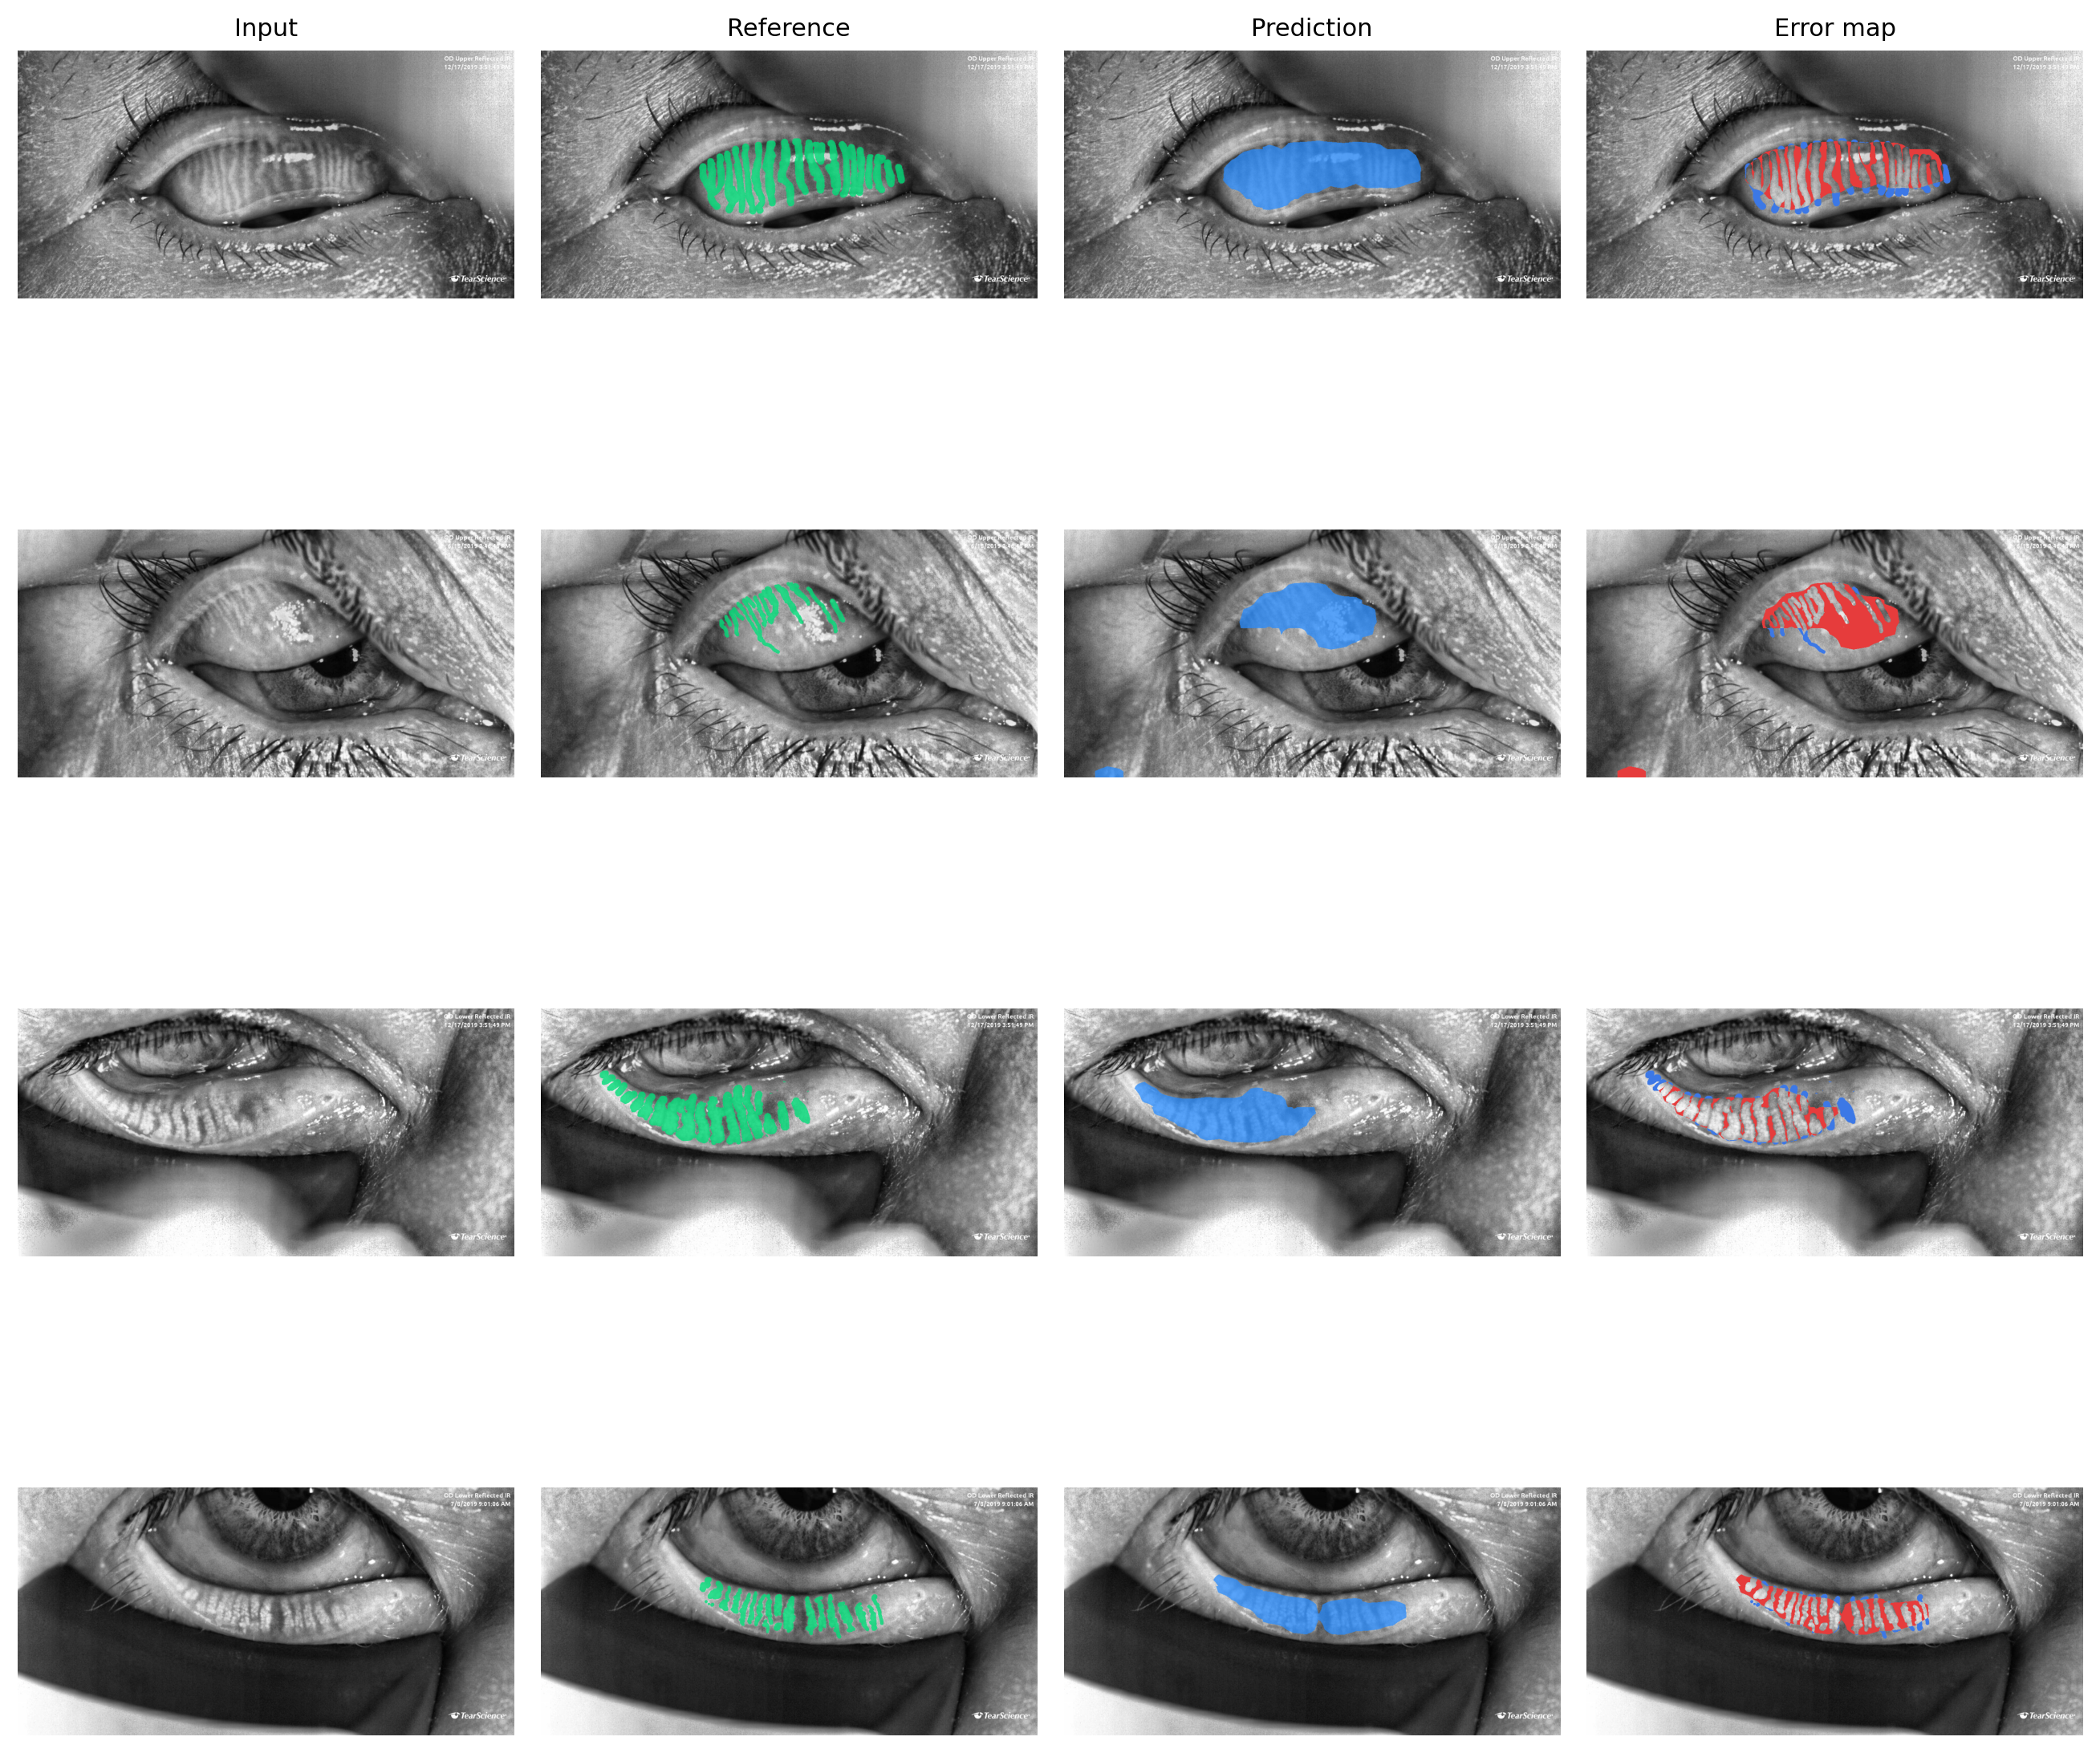
\includegraphics[width=\linewidth]{figures/qualitative.png}
\caption{定性结果：输入、专家参考、模型预测与错误图（红为假阳性，蓝为假阴性）。行按上/下睑选取；错误图用于展示断裂、粘连与睑缘外漏的形态，而不是替代指标。}
\label{fig:qualitative}
\end{figure}


\subsection{旧权重的工程回归}

旧 UNet 权重来自对全部 \nTotal{} 例随机打乱、无 holdout 的训练脚本，因此其“测试”指标可能是训练集自评，且官方 200 例测试名单可能在其训练数据中。本文只把它作为工程回归锚点：Dice \legacyUNetSelfDice、IoU \legacyUNetSelfIoU、clDice \legacyUNetSelfClDice。该数字\textbf{不得}进入独立测试表，也不得与本文其他模型比较。

\subsection{讨论}

把上述结果放在一起，本文的论点不是“某个主干全面胜出”，而是三件事：第一，患者级划分会改变结论，公开基准必须报告派分签名；第二，分块是与主干同等级的实验变量，MTE 提供了一种不重训的稳定化手段；第三，像素指标与临床分级必须同时报告，否则“分割更好”可能不等于“分级更准”。这三件事都比再增加一个 backbone 更接近临床可用的证据。

\section{局限性与风险}\label{sec:limitations}

\paragraph{单中心、单设备的公开数据。}MGD-1K 来自 LipiView II，320 名受试者；本文的患者级划分只能保证受试者不跨 split，不能保证跨设备或跨中心泛化。2025 年的多中心工作已经说明，设备与人群差异会实质影响性能\cite{li2025multicenter}；本文没有外部多中心测试集，因此不能声称临床泛化。

\paragraph{9 小时预算与单次 holdout。}本轮为控制总预算采用单次患者级 holdout，而非 5 折交叉验证；部分模型（尤其 WRCANet 与 MGD-PriorNet）未完全收敛。结果应定位为“可复现的初步证据”，不能声称最优；5 折与更多 epoch 是后续工作。

\paragraph{泄漏对照的统计功效有限。}clean-official 子集只有 \cleanOfficialImages{} 图/\cleanOfficialPatients{} 患者，足以展示泄漏方向，但不足以给出稳定的临床结论。leaky 与 patient-level 的差值应结合置信区间解读，不能只看点估计。

\paragraph{临床终点仍不完整。}本文的临床一致性只到 Meiboscore；没有症状评分、睑板挤压、分泌物质量或前瞻性随访。分割指标的提升是否转化为诊断或治疗决策收益，需要独立的前瞻性研究。

\paragraph{距离指标缺少物理标定。}影像没有 mm/pixel 标定，HD95 与 ASSD 的单位是像素；不同设备、不同原始分辨率缩放到 $640\times1280$ 后不可直接比较。R\_loss 与 Meiboscore 基于像素比例，只能作为比例参考值。

\paragraph{预训练可能降级。}MGD-Former 的编码器默认从 ADE20K 权重初始化；目标机器离线且本地无缓存时会退化为随机初始化，run 元数据与日志会记录 \texttt{pretrained\_status} 与原因。若最终结果来自随机初始化，必须如实标注。

\paragraph{协议边界。}本文的架构比较只在本数据、本预处理、本患者级划分与本推理配置下有效。换数据、换设备或换分块，排序可能改变。本文不主张“某架构普遍更优”，也不把单一数据集的显著性当作临床有效性证据。

\paragraph{旧权重的数据泄漏。}旧 UNet 权重对全部 \nTotal{} 例做过随机打乱，没有留出测试集；它只能作为工程回归锚点，不能作为独立测试性能，也不能与本文其他模型比较。

\paragraph{许可与伦理。}MGD-1K 为公开数据集，但其许可与再分发条款需在投稿前再次核验；本文不声明超出数据集原始许可的再分发权。

\section{结论}\label{sec:conclusion}

本文把睑板腺红外影像分割的问题从“再设计一个分割网络”转为“建立可比较、可审计的证据”。在公开 MGD-1K 上，我们建立了患者级划分（\nTrain/\nVal/\nTest{} 图像，\nTrainPatients/\nValPatients/\nTestPatients{} 名患者），并同时记录文件清单签名与派分签名；这使得“同名文件、不同派分”不再是不可追溯的隐性变量。

方法学上，本文给出三项可复用的发现。第一，泄漏是可量化的：官方 \officialTestImages{} 例 Meiboscore 测试清单来自 \officialTestPatients{} 名患者，其余 800 例中有 \officialLeakImages{} 例来自同一批患者；即使患者级训练集也仍含 \officialLeakPatients/\officialTestPatients{} 名测试患者。第二，分块是与主干同等级的实验变量：同一权重仅改分块高度，Dice 可从 0.370 变到 0.655；MTE 用 256/384/512 三个分块的概率平均，在本轮主要改善 HD95（68.05→61.85）而非 Dice，因此定位为边界校正而非涨点方法。多分块方差的失败检测 AUROC 仅 0.639，TTA8 的 1.000 受标签--信号耦合影响，二者都不足以单独作为 triage 规则。第三，像素指标与临床终点必须同时报告：本队列中分割导出的 Meiboscore 与专家分级的 QWK 仅 0.131，说明当前 R\_loss→Meiboscore 链条不足以替代专家分级；上/下睑也必须分开报告。

架构上，MGD-Former 用 MiT-B2 编码器保留 1/4 特征，以融合解码器输出 stride=4，并在三个尺度深监督；ADE20K 预训练针对 \nTotal{} 例的小数据冷启动。它是五条路线之一，而不是本文的唯一卖点。本文不提供未经实测的精度结论；所有数值已从统一训练与患者级独立测试的结果文件注入，并以置信区间、配对检验与多指标（Dice、clDice、HD95、ASSD、临床 QWK）共同支撑。

\section*{声明}
\addcontentsline{toc}{section}{声明}

\subsection*{伦理与知情同意}
本研究使用的影像数据为脱敏回顾性数据。伦理批号、批准机构与知情同意方式均为待填项：\needcheck{伦理批号与批准机构}。若数据来自公开数据集，需在此写明数据集名称、版本、许可与获取日期；若来自院内采集，需写明豁免知情同意的依据。

\subsection*{数据可得性}
数据受伦理与再分发许可限制，暂不公开原始影像。去标识化的划分清单、\path{split_signature}、评测脚本与结果文件可在合理请求下提供；MGD1k 的许可条款待核验，未确认前不声明可再分发。

\subsection*{代码与权重可得性}
训练与推理内核、配置 schema、评测与统计脚本、图表生成脚本构成可复现包，版本 2.3.0。权重发布前需完成 \texttt{verified} 转正流程；未验证权重不作为正式发布物。权重 manifest 含 SHA-256、输入尺寸、归一化口径与训练来源。

\subsection*{利益冲突}
作者声明无经济利益冲突。\needcheck{如涉及设备厂商或数据提供方合作，需在此披露}

\subsection*{资助}
基金名称、编号与资助范围待填：\needcheck{基金信息}。

\subsection*{作者贡献}
概念与设计、数据采集与标注、模型与工程实现、实验执行、统计分析与稿件撰写的人员分工待填。\needcheck{CRediT 贡献列表}

\subsection*{生成式工具使用声明}
若在稿件准备中使用生成式工具，仅用于语言润色与排版检查，不用于生成数据、结果或参考文献；所有引用均经人工核验。


\bibliographystyle{unsrt}
\bibliography{refs}

\appendix
\section{可复现性清单}\label{app:checklist}

本附录按 CLAIM 与 REFORMS 的结构给出可核对项。表中“状态”为本文当前的完成度；“待完成”项必须在投稿前补齐。

\begin{table}[h]
\centering
\caption{可复现性清单。}
\label{tab:checklist}
\small
\begin{tabular}{p{0.34\linewidth}p{0.42\linewidth}p{0.14\linewidth}}
\toprule
项目 & 本文做法 & 状态 \\
\midrule
数据来源与许可 & 公开 MGD-1K（1000 图 / 320 受试者 / LipiView II）；内容级去重后 \nTotal{} 例；许可与再分发条款投稿前复核 & 已实现，许可待核 \\
患者级划分 & \nTrain/\nVal/\nTest{} 图像；\nTrainPatients/\nValPatients/\nTestPatients{} 名患者；患者互斥 & 已实现 \\
签名 & 文件清单签名 \splitSig{} + 实际派分签名 \assignmentSig{} & 已实现 \\
泄漏审计 & 官方 200 图/\officialTestPatients{} 患者；\officialLeakImages/800{} 图像级泄漏；\officialLeakPatients/\officialTestPatients{} 患者级泄漏；clean-official \cleanOfficialImages{} 图/\cleanOfficialPatients{} 患者 & 已实现 \\
预处理口径 & 五步固定管线；训练/推理逐像素一致 & 已实现 \\
模型与损失 & MGD-Former + 四基线；统一损失组合 & 已实现 \\
训练配方 & AdamW/余弦/AMP/EMA 0.99/增强/多尺度；每模型 epochs 见表~\ref{tab:ablation-design} & 已实现 \\
推理参数 & 分块 $384\times768$、重叠 0.25、阈值 0.7 & 已实现 \\
分块敏感性 & 7 个实测点；同权重、仅改分块 & 已实测 \\
MTE 与不确定性 & 256/384/512 概率平均；方差/熵/TTA 的 AUROC & 已实现，数值待注入 \\
临床分级 & 分割→R\_loss→Meiboscore 与 6 轮专家分级的 accuracy/MAE/QWK & 已实现，数值待注入 \\
显存档位 & 6/8 实测；12--40 GB 估算 & 部分实测 \\
统计协议 & bootstrap 1000；Wilcoxon + Holm & 已实现 \\
精度结果 & 9 小时统一训练与 patient-level 独立测试；数值见结果表 & 已实现 \\
权重状态 & \texttt{verified=false} 草稿；转正需独立评估 & 待完成 \\
\bottomrule
\end{tabular}
\end{table}

\section{超参数与实现细节}\label{app:hyper}

\begin{table}[h]
\centering
\caption{训练与推理默认配置（唯一来源为工程的参数 schema）。}
\label{tab:hyper}
\small
\resizebox{\linewidth}{!}{%
\begin{tabular}{lll}
\toprule
分节 & 参数 & 默认值 \\
\midrule
run & seed / 设备 & 42 / 自适应（CUDA、CPU） \\
data & 输入尺寸 / 划分 & $640\times1280$ / patient-level \nTrain/\nVal/\nTest \\
model & 主干 / 预训练 / 输出通道 & MGD-Former / ADE20K / 2 \\
train & 优化器 / 学习率 / 权重衰减 & AdamW / $1\times10^{-4}$ / $1\times10^{-4}$ \\
train & 调度 / warmup / 轮数 & cosine / 5\% / 45（主模型；其余见表~\ref{tab:ablation-design}） \\
train & EMA / AMP / 梯度累积 & 0.99 / CUDA 开 / 1（WRCANet 2） \\
train & 分块 / batch / channels\_last & $384\times768$ / 4（WRCANet 2） / 是 \\
train & 深监督权重 & 1.0 / 0.5 / 0.25 \\
loss & Dice / CE / clDice / 睑缘 & 0.4 / 0.4 / 0.2（10\% warmup）/ 0.25 \\
eval & 分块 / 重叠 / 阈值 & $384\times768$ / 0.25 / 0.7 \\
eval & MTE / TTA & 256/384/512 概率平均 / 关闭或 8 倍 \\
clinical & Meiboscore & 6 轮专家分级多数票；accuracy/MAE/QWK \\
\bottomrule
\end{tabular}}
\end{table}

\section{构建与复现命令}\label{app:build}

中文版使用 XeLaTeX 与 ctex（\texttt{fontset=windows}），英文版使用 pdfLaTeX。两版的编译顺序均为：首次编译 → BibTeX → 两次编译。图~\ref{fig:tiling}、图~\ref{fig:vram} 与图~\ref{fig:pipeline} 的数值来自 \texttt{data/results.tex} 的宏，正文与图共用同一宏源；真实结果注入后只需修改该文件。

环境依赖：Python $\ge$ 3.10、torch 2.5.1、numpy 1.26.4、opencv-python 4.8+、scikit-image 0.25.2、monai 1.5.2、scipy 1.15.3。数据准备、训练与评估命令见工程 Runbook；本文不重复粘贴，以避免版本漂移。


\end{document}
